%************************************************
\chapter{Image Decomposition}\label{ch:decomposition}
%************************************************

In this chapter, we will focus on those \ac{CAD} systems that use a combination of an image decomposition method and feature selection by means of hypothesis testing. These variety of methods have been published in \cite{Martinez201141,Martinez-Murcia20129676,Martinez-Murcia2013255,Martinez-Murcia201458}. 

Image decomposition methods model a set of samples as a linear combination of $c$ latent variables, also known as components. These variables can be considered as the basis of a $c$-dimensional space where each sample is represented by a feature vector of length $c$. The $i$-th neuroimage in our dataset can be therefore decomposed as: 

\begin{equation}\label{eq:generalDecomposition}
	\mathbf{x}_i = s_0 \mathbf{w}_0 + s_1 \mathbf{w}_1 + \dots + s_c \mathbf{w}_c + \boldmath\epsilon = \mathbf{s}\mathbf{W} + \boldmath\epsilon
\end{equation}

Where $s_i$ is the coordinate (or component score) of the current image in the $i$-th dimension of the new space defined by all the base vectors $\mathbf{w}_i$ (component loadings), and $\boldmath\epsilon$ is the error of the estimation. Figure \ref{fig:decomposition_overview} shows an illustration of the process. 

\begin{figure}[tph]
	\centering
	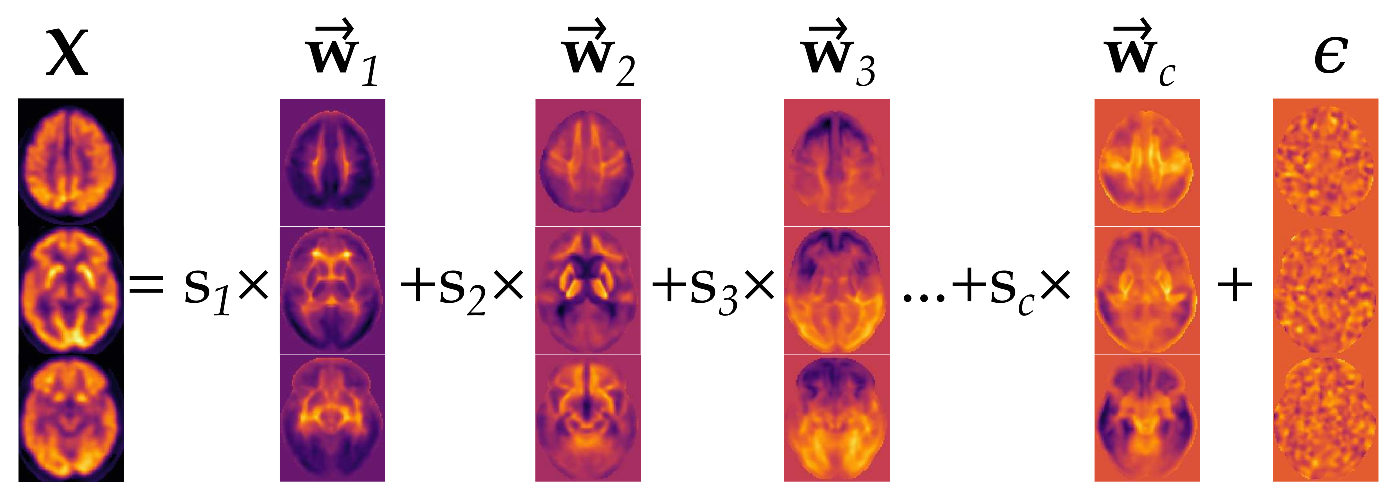
\includegraphics[width=0.9\linewidth]{Graphics/ch4/decomposition_overview}
	\caption[Illustration of how decomposition algorithms work.]{Illustration of how decomposition algorithms such as \ac{FA} and \ac{ICA} work on a \ac{PET}-FDG brain image.}
	\label{fig:decomposition_overview}
\end{figure}

Many signal decomposition techniques are used in the literature, for example \ac{PCA} or \ac{PLS} \cite{Spetsieris2009,Illan2011,Towey2011,Segovia2013,Khedher2015}. We will focus on two less known decomposition algorithms \acf{FA} and \acf{ICA}, which we will integrate in different \ac{CAD} systems using a pipeline similar to the one displayed at Figure~\ref{fig:pipelineDecomposition}. This pipeline involves feature selection (for reducing the dimensionality), decomposition of the feature vectors and classification.
 
\begin{figure}[tph]
	\centering
	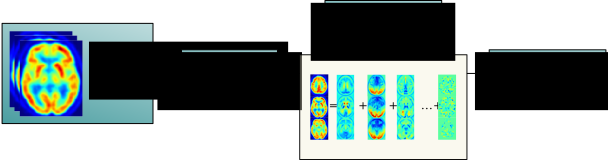
\includegraphics[width=0.7\linewidth]{Graphics/ch4/01-flowdiagram}
	\caption[Illustration of the system used in Chapter~\protect\ref{ch:decomposition} .]{Illustration of the system used in Chapter~\protect\ref{ch:decomposition}.}
	\label{fig:pipelineDecomposition}
\end{figure}

\section{Feature Selection}
Feature selection is the first strategy used for feature reduction \cite{Martinez-Murcia2016b}, and it is often used along with feature extraction in order to build more complex pattern recognition systems. It refers to any strategy intended to find a subset of the original features containing the more suitable ones according to a certain criterion. Therefore, irrelevant features are discarded, and resultant models are faster and more cost-effective \cite{Guyon03}. However, it usually requires an additional optimization to find the parameters for the optimal feature subset, and furthermore, it is impossible to guarantee that the optimal features for the subset are the same of the full feature set \cite{DaelemansHosteMeulderEtAl2003}. 

In this work, we will use filtering methods to perform feature selection. As we introduced in Section~\ref{sec:mvanalyses}, filtering methods are based on the computation of a feature relevance score directly on the data. The relevance score is used to sort the different features, discarding those with a lower score, and it is usually computed independently for each feature, in what is called a univariate approach \cite{SaeysInzaLarranaga2007}. 

Feature selection can be used before or after feature extraction. When using computationally-intensive algorithms such as \ac{FA} or especially \ac{ICA}, the selection of best features prior to the decomposition is key to obtain high performance while keeping the computation times small \cite{Martinez201141,Martinez-Murcia20129676}. This also removes noise in some cases where the decomposition algorithm cannot compute correctly the variance. 

\begin{figure}[bth]
	\myfloatalign
	\subfloat[$t$-test.]
	{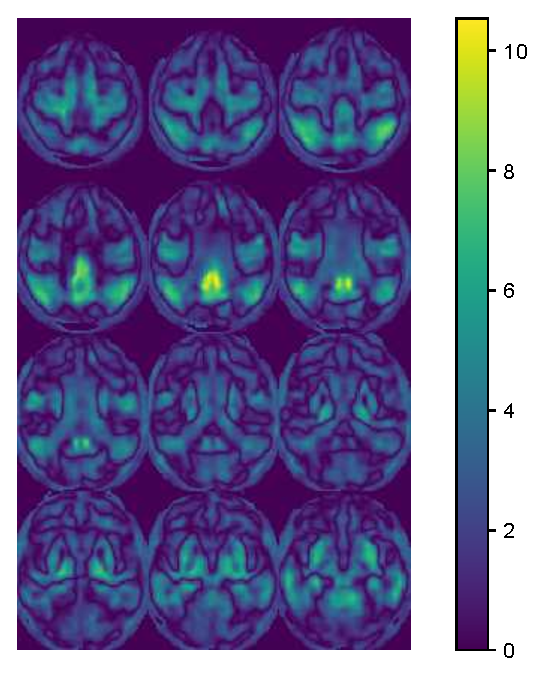
\includegraphics[width=.3\linewidth]{Graphics/ch4/ttest_map.eps}\label{fig:ttest_map}}\quad
	\subfloat[\ac{KL} divergence.]
	{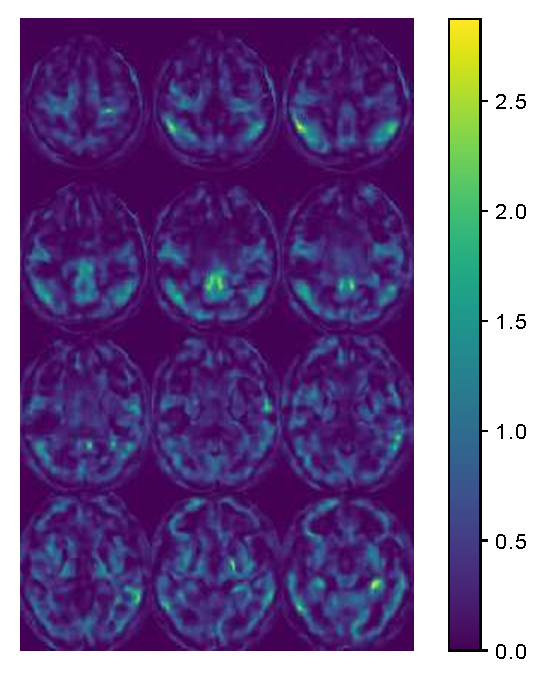
\includegraphics[width=.3\linewidth]{Graphics/ch4/kl_map.eps}\label{fig:kl_map}}\quad
	\subfloat[\ac{MWW} $U$-test.]
	{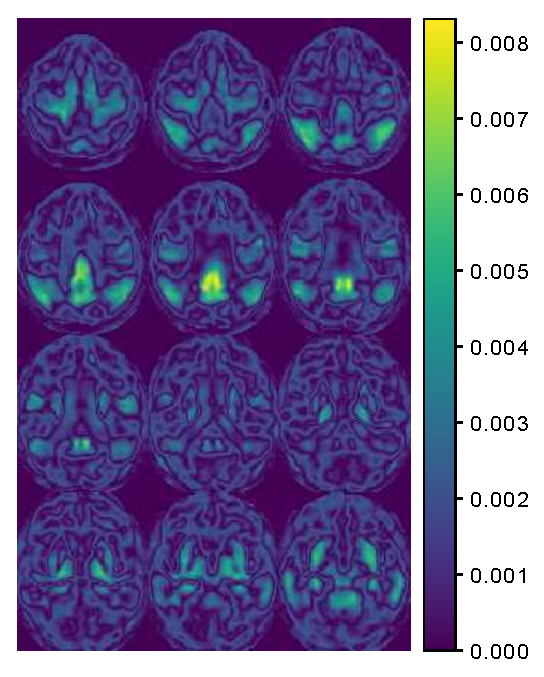
\includegraphics[width=.3\linewidth]{Graphics/ch4/wilcoxon_map.eps}\label{fig:wilcoxon_map}}
	\caption[Comparison between the different filtering methods.]{Comparison between the different filtering methods, and the regions selected by them, in the ADNI-PET dataset. }\label{fig:comparisonSelection}
\end{figure}

Three feature selection algorithms have been used in this thesis, not only in the \ac{CAD} systems proposed in this chapter, but in many other models that will be presented later: the $t$-Test, the Kullback-Leibler divergence or Relative Entropy, and the Mann-Whitney-Wilcoxon rank test. 

\subsection{$t$-test}
The $t$-test is an old friend of statisticians. In this work we will use the independent two-sample $t$-test \cite{Fay10}. It quantifies the differences between two classes using an assumption of independent variances. Let $X_i^f$ a vector containing the $f$-th feature of all elements in class $i$. The $t$-score of the $f$-th feature can be computed as:

\begin{equation}
t_f = \frac{\bar{X}_1^f - \bar{X}_2^f}{\sqrt{\frac{\sigma_{X_2^f}^2+\sigma_{X_1^f}^2}{n}}}
\end{equation}
where $\sigma_{X_i^f}^2$ is the variance and $\bar{X}_i^f$ is the average of the $f$-the feature within class $i$. The $t$-test is extensively used in the neuroimaging community, and it is the basis for the \ac{SPM} and \ac{VBM} analyses \cite{spm_book}. See figure~\ref{fig:ttest_map} for an example of the $t$-test computed on the ADNI-PET database.

\subsection{Kullback-Leibler Divergence} 
Another alternative is the \acf{KL} divergence, also known as Relative Entropy. It is a non-symmetric measure of the difference between two probabilities distributions. Let us assume that $X_1^f$ and $X_2^f$, the vectors containing the $f$-th feature of all elements in class $i$, are two discrete random variables. Therefore, the \ac{KL} divergence can be calculated with equation \ref{kullback} \cite{Theodoridis1999}.

\begin{equation}\label{kullback}
KL_f = \left(\frac{\sigma_{X_2^f}^2}{\sigma_{X_1^f}^2} +\frac{\sigma_{X_1^f}^2}{\sigma_{X_2^f}^2} -2 \right) + \frac{1}{2}\left(\bar{X}_2^f-\bar{X}_1^f\right)^2\left(\frac{1}{\sigma_{X_1^f}^2} + \frac{1}{\sigma_{X_2^f}^2}\right)
\end{equation}
using the same notation than in $t$-test. See figure~\ref{fig:kl_map} for an example of the computed \ac{KL} divergence on the ADNI-PET database.

\subsection{Mann-Whitney-Wilcoxon} 
The \acf{MWW} rank test, also known as $U$-test, assigns a rank to all values in the vector corresponding to the $f$-th feature, $X^f$, without considering any class. The method used to assign a rank is the `average', which means that each value is assigned with the average of the ranks that would have been assigned to all the tied values. This means that, for example, in the case of the vector $X^f=(0,2,3,2)$, the ranks assigned to each element would be $R^f=(1,2.5,4,2.5)$. 

Let $n_1$ and $n_2$ be the number of elements in class 1 and 2 respectively, and $R^f$ the vector of ranked elements. We proceed by selecting the first $n_1$ elements in $R^f$ by: 
\begin{equation}
	R^f_{n_1} = {R^f_i} \quad \forall i\in(0,n_1)
\end{equation}

The $U$-score for the $f$-th feature and the first class will be: 
\begin{equation}
	U_1^f = n_1 n_2 + n_1 \frac{n1+1}{2} - \sum R^f_{n_1}
\end{equation}

And the it can be computed for the second class as the remainder: 
\begin{equation}
	U_2^f = n_1 n_2 - U_1
\end{equation}

The final $U^f$ can be assigned to either $U_1^f$, $U_2^f$ or $\min{U_1^f,U_2^f}$ \cite{Fay10}, but the usual approach nowadays is to assign $U^f=U_2^f$. Unlike $t$-test, \ac{MWW} test does not assume any prior distribution, and therefore is less likely than it to spuriously indicate significance because of the presence of outliers. Under the normal distribution, it performs relatively similar \cite{Fay10}. See figure~\ref{fig:wilcoxon_map} for an example of the \ac{MWW} $U$-test computed on the ADNI-PET database.

\section{Decomposition Algorithms}
The feature selection algorithms presented above will perform a significant feature reduction, from hundreds of thousands of voxels to a few thousands. These few thousands voxels are considered the best in discriminating between \ac{CTL} and affected subjects in each of the diseases. The feature selection strategy can be thought of as a mask, in which only the most relevant regions according to the tests are selected (see Figure~\ref{fig:comparisonSelection}). 

However, this number of features is still large, and therefore, further feature reduction can be applied by performing a decomposition of the masked regions. We have used two algorithms in our \ac{CAD} systems: \acf{FA} and \acf{ICA}.

\begin{figure}[bth]
	\myfloatalign
	\subfloat[Original]
	{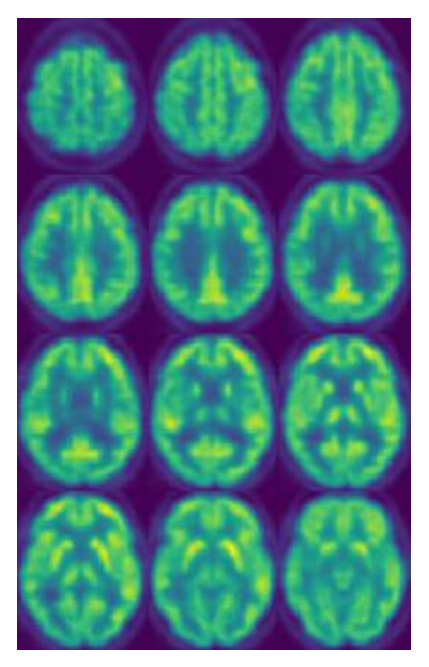
\includegraphics[width=.3\linewidth]{Graphics/ch4/originalImage.eps}}\quad
	\subfloat[\ac{FA} reconstruction]
	{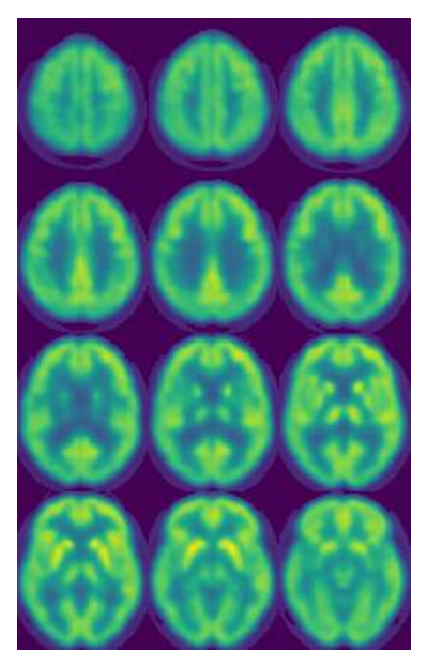
\includegraphics[width=.3\linewidth]{Graphics/ch4/transformedFA.eps}}\quad
	\subfloat[\ac{ICA} reconstruction]
	{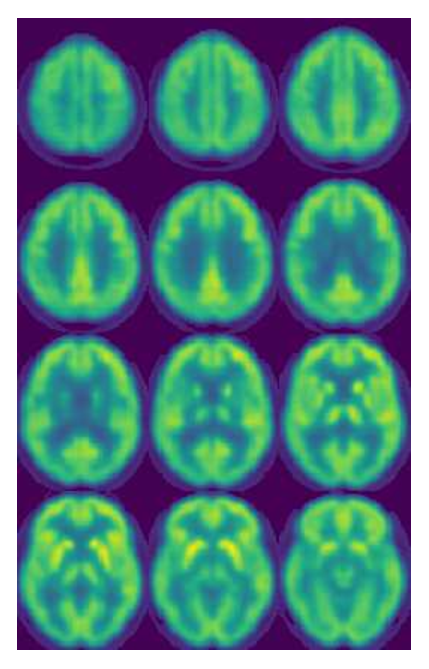
\includegraphics[width=.3\linewidth]{Graphics/ch4/transformedICA.eps}}
	\caption[Original PET image and its reconstruction using FA or ICA.]{Original PET image from the ADNI-PET dataset, and examples of reconstruction using \ac{FA} or \ac{ICA}, with 10 components.}\label{fig:comparisonReconstructions}
\end{figure}


\subsection{Factor Analysis}
\acf{FA} was used in \cite{Martinez201141,Martinez-Murcia20129676} to perform feature extraction in \ac{CAD} systems. This strategy assumes that each image in the database is a realization of a given experiment. \ac{FA} then models each of the $N$ observations (or subjects) as the expression of $c$ unobserved variables, known as factors. The model follows the general decomposition equation (Eq. \ref{eq:generalDecomposition}), but assuming that the dataset matrix $\mathbf{X}$ is zero-centred. That is, that we have subtracted the mean prior to the computation. In matrix form, Eq. \ref{eq:generalDecomposition} can be rewritten as:

\begin{equation}\label{eq:factoranalysis}
\mathbf{X} -\boldsymbol{\mu}= \mathbf{S}\mathbf{W} +  \boldsymbol{\epsilon}
\end{equation}

The columns of $\mathbf{W}$ are known as factors, and the rows of $\mathbf{S}$ are known as loadings  (similar to the concept of component loading and component scores in \ac{PCA}). Thanks to this, we can convert the original dataset $\mathbf{X}$ of size $N\times f$ into $\mathbf{S}$, of size $N\times c$. The procedure of computing the decomposition imposes some assumptions on $\mathbf{W}$: 
\begin{itemize}
	\item $\mathbf{W}$ and $\boldsymbol{\epsilon}$ must be independent. 
	\item $E[\mathbf{W}] = 0$. 
	\item $\text{Cov}(\mathbf{W}) = \mathbf{I}$, which ensures that the factors are uncorrelated. 
\end{itemize}

Now we can rewrite Eq.~\ref{eq:factoranalysis} as:
\begin{equation}\label{eq:fastep1}
	\text{Cov}(\mathbf{X} -\boldsymbol{\mu})= \text{Cov}(\mathbf{S}\mathbf{W} +  \boldsymbol{\epsilon})
\end{equation} 

Under the previous constraints, and setting $\boldsymbol{\Sigma} = \text{Cov}(\mathbf{X} -\boldsymbol{\mu})$, Eq.~\ref{eq:fastep1} becomes:
\begin{equation}
	\boldsymbol{\Sigma} = \mathbf{S}\text{Cov}(\mathbf{W})\mathbf{S}^T - \text{Cov}(\boldsymbol{\epsilon})
\end{equation}

Since $\text{Cov}(\mathbf{W}) = \mathbf{I}$, and making $\text{Cov}(\boldsymbol{\epsilon})=\boldsymbol{\Psi}$, the diagonal matrix containing the specific variances of the reconstruction error, we obtain the alternative form of \ac{FA}: 
\begin{equation}
\boldsymbol{\Sigma} = \mathbf{S}\mathbf{S}^T - \boldsymbol{\Psi}
\end{equation}

The mean $\boldsymbol{\mu}$, and the matrices $\mathbf{S}$ and $\boldsymbol{\Psi}$ are obtained via Maximum Likelihood estimation. To guarantee an unique solution, we impose that $\mathbf{S}^T\boldsymbol{\Psi}^{-1}\mathbf{S}$ is a diagonal matrix. Then, we obtain the parameters by maximizing the log-likelihood given by the following expression: 
\begin{equation}
	\ell(\mu,\mathbf{S},\boldsymbol{\Psi}) = - \frac{np}{2}\log{2\pi}- \frac{n}{2}\log{\left|\mathbf{SS}^T + \boldsymbol{\Psi}\right|} - \frac{1}{2}\sum_{i=1}^{n}(\mathbf{x}_i-\mu)^T(\mathbf{SS}^T+\boldsymbol{\Psi})(\mathbf{x}_i-\mu)
\end{equation} 

\ac{FA} differs from \ac{PCA} mainly because it performs an estimation of the noise, and needs the number of factors $c$ as an input. Choosing $c$ is not a naive task. A large $c$ can yield a small reconstruction error, but the factors will not be representative enough, leading to overfitting of the subsequent model. Conversely, a small $c$ can lead to a large reconstruction error, causing information loss. We have computed the reconstruction error variance over the ADNI-PET dataset, and plotted it in Figure~\ref{fig:error} (similar graphs can be obtained for other databases. This proves that the error is assymptotical as we increase $c$, and therefore, once arrived at certain error, the improvements are not significant. 

\begin{figure}[ht]
	\centering
	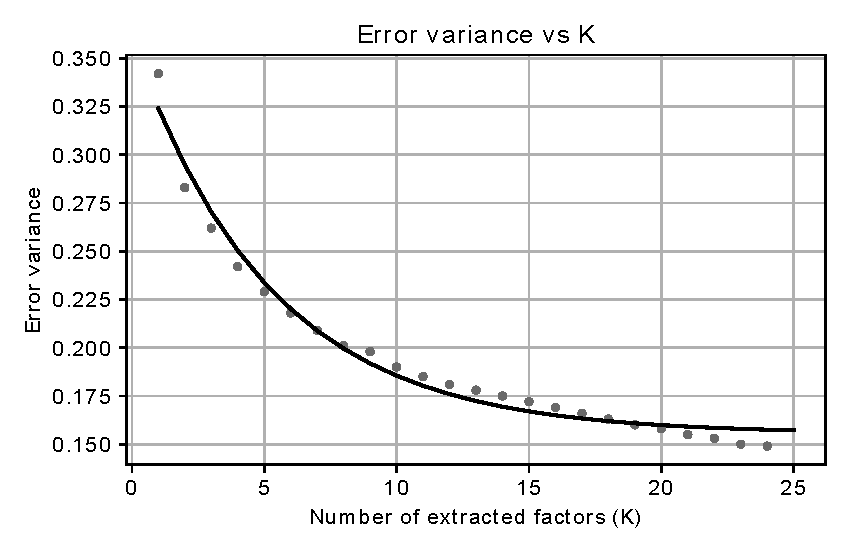
\includegraphics[width=0.5\linewidth]{Graphics/ch4/varError-K-ADNI}
	\caption{Specific variance of reconstruction error $\Psi$ using \ac{FA}, in function of number of factors extracted ($K$) for ADNI-PET database (the behaviour is similar in other datasets).}
	\label{fig:error}
\end{figure}


\subsection{Independent Component Analysis}
\cite{Martinez-Murcia2013255,Martinez-Murcia201458}

\acf{ICA} \cite{Hyvarinen2000}, is a statistical technique that represents a multidimensional random vector as a lineal combination of non-gaussian random variables (the so-called ''independent components'') to be as independent as possible, and has been used widely on segmentation and clustering of medical images \cite{DeMartino2007,Alvarez2009}. It can be considered as a non-gaussian version of Factor Analysis. Assume that we observe $n$ lineal mixtures $\mathbf{x}_1, \mathbf{x}_2, \ldots, \mathbf{x}_n$ of length $N$ that can be modelled as an expression of $K$ independent components (IC). These independent components are defined as $\mathbf{S} = (\mathbf{s}_1, \mathbf{s}_2, ... \mathbf{s}_K)$, where each $\mathbf{s}_K$ vector has a length of $N$. So, each random vector $\mathbf{x}_n$ can be described as a linear combination of $K$ independent components: 

\begin{equation}
\mathbf{x_n} = a_{1n}\mathbf{s}_1 + a_{2n}\mathbf{s}_2 + \ldots + a_{Kn}\mathbf{s}_K
\end{equation}

Without loss of generality we can assume that both the observed vectors and the independent components are are zero mean. If the previous conditions are not met, the $\mathbf{x}$ variables can be centered by subtracting the sample mean. To use a vector-matrix notation, more convenient in this case, we denote as matrix $\mathbf{X}$ the random vector whose elements are $\mathbf{x}_1, \ldots, \mathbf{x}_n$. We also denote as $\mathbf{A}$ the matrix that contains all $a_{Kn}$ elements, the ''mixing matrix'' that projects each image into the space defined by the IC. Using this notation, the mixing model above remains as follows: 

\begin{equation}\label{eq:ica}
\mathbf{X}=\mathbf{A}\mathbf{S}
\end{equation}

The starting point of ICA is the assumption that all components $\mathbf{s}_K$ are are statistically independent. To measure independence, we assume that all independent components have a non-gaussian statistical distribution. It is assumed that a sum of independent signal trends to gaussianity, so if non-gaussianity is maximized with any independence criteria $F$, for instance, the kurtosis or negentropy, we obtain signals that are more independent than the previous ones \cite{Hyvarinen1999,Hyvarinen2000}.
After estimating the matrix $\mathbf{A}$, we can compute its inverse, $\mathbf{W}$ and obtain the projection $\mathbf{S}$ of the images in the dataset into the IC space with: 
\begin{equation}
\mathbf{S} = \mathbf{W}\mathbf{X}
\end{equation}

\subsubsection{FastICA}
Adaptive algorithms based on gradient descend can be problematic when they are used on an environment in which adaptation is not necessary, like this case. The convergence is often slow, and depends on the choice of convergence parameters. As a solution to this problem, block algorithms based on fixed-point iteration \cite{Oja1997,FastICA99} can be used. In \cite{Oja1997} a fixed-point algorithm based on kurtosis is introduced. In \cite{FastICA99}, this algorithm, known as FastICA, is generalized to general contrast functions. The single unit FastICA algorithm has the following form:
\begin{equation}
\mathbf{w}(k) = E\lbrace\mathbf{x}g(\mathbf{w}(k-1)^T\mathbf{x})\rbrace -E\lbrace g'(\mathbf{w}(k-1)^T\mathbf{x})\rbrace\mathbf{w}(k-1)
\end{equation}
where the loadings vector $\mathbf{w}$ is normalized to unit norm in each iteration, and the function $g(x)$ is a derivative of the contrast function $G$ defined in \cite{Hyvarinen1999}. The expected values are estimated in practice by using the mean of a significantly high number of samples of the input data. 
The speed of convergence of the fixed-point algorithms is clearly superior to more neural algorithms. Improvements between 10 and 100 times the speed are observed frequently \cite{Giannakopoulos1998}. 


% AQUÍ EMPIEZA LO QUE HEMOS ESCRITO YA. 
\section{Results}
In this work we will analyse the behaviour of the system proposed in the introduction and illustrated at Figure~\ref{fig:pipelineDecomposition}. The system comprises the selection of the most relevant voxels using filtering methods (we will focus on $t$-test, relative entropy and wilcoxon) and a feature decomposition of these using either \ac{FA} or \ac{ICA}. Finally, the feature vectors are classified using a \ac{SVC} with linear kernel, and performance values are obtained via cross-validation (see Section~\ref{sec:validation} for more information). 

We vary the number of selected voxels and the number of factors or components depending on the algorithm and the dataset used and evaluate the system with those characteristics. That way, we obtain an estimation of the performance of the system in different situations, so that we can draw conclusions on the disease patterns and the ability of the system in the detection of different diseases. 

\subsection{Alzheimer's Disease}
We begin by applying the proposed feature selection plus decomposition pipeline to the two functional neuroimaging datasets: ADNI-PET and VDLN-HMPAO. For this experiment we will use a maximum of $20,000$ selected voxels and $25$ components. 

\subsubsection{Factor Analysis}\label{sec:results_FA_AD}
First, we use \ac{FA} as a decomposition technique. In Figure~\ref{fig:accuracyMeanFA-AD} we average the accuracy over the number of voxels or the number of components respectively, to look at how these variables affect the performance of the system, and we do this for the three filtering methods used. 

\begin{figure}	\centering
	\subfloat[]{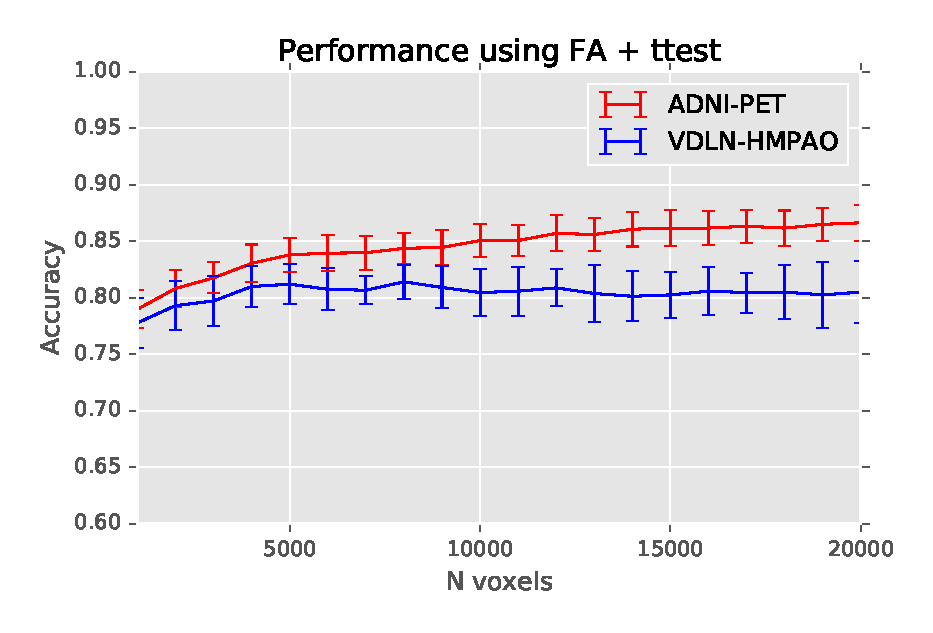
\includegraphics[width=0.49\linewidth]{Graphics/ch4/accuracyMeanSTD-FA_vsN_ttest_AD.eps}\label{fig:AD-AV-FA-TTEST-VSN}}
	\subfloat[]{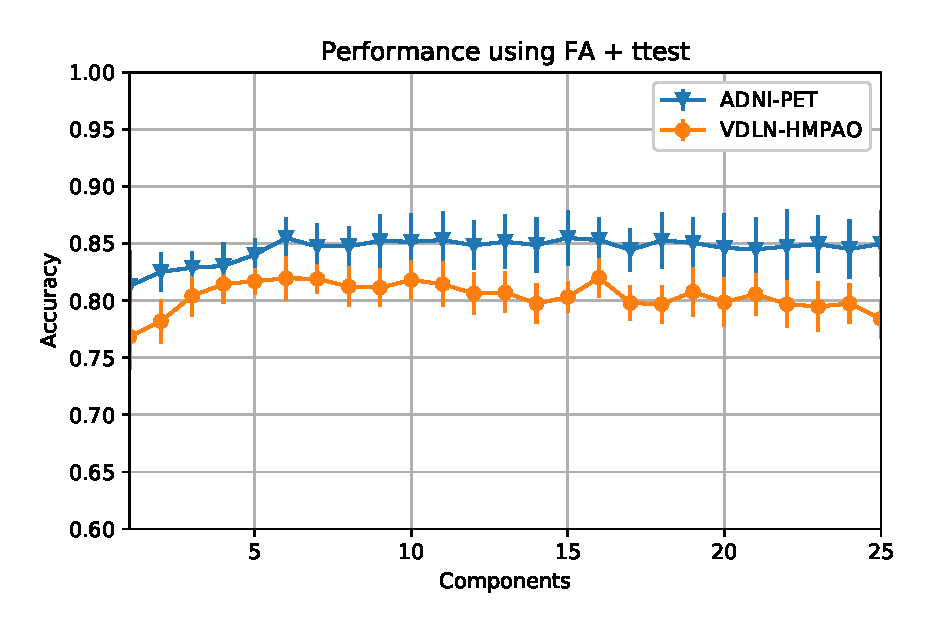
\includegraphics[width=0.49\linewidth]{Graphics/ch4/accuracyMeanSTD-FA_vsK_ttest_AD.eps}\label{fig:AD-AV-FA-TTEST-VSK}}
	
	\subfloat[]{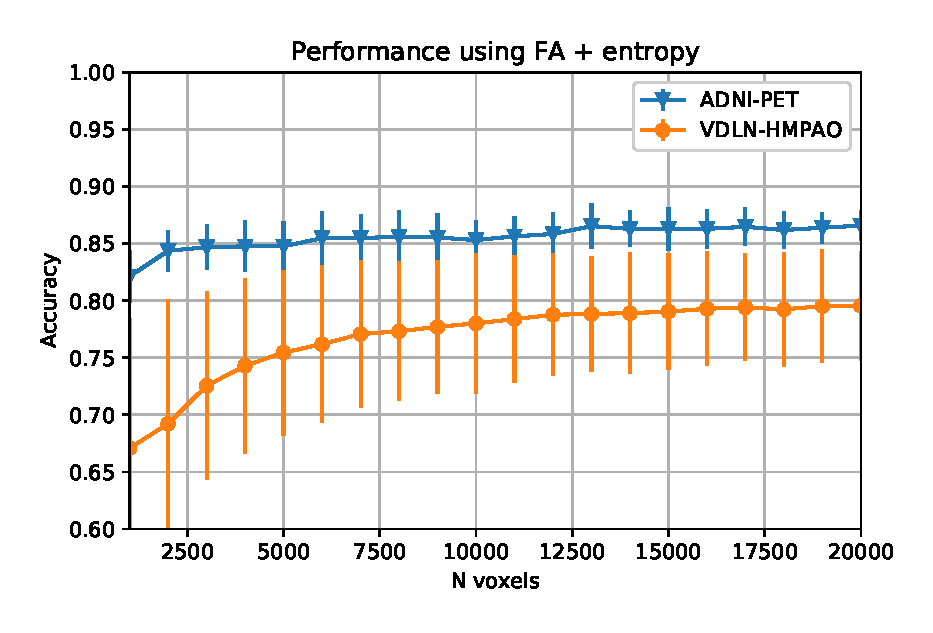
\includegraphics[width=0.49\linewidth]{Graphics/ch4/accuracyMeanSTD-FA_vsN_entropy_AD.eps}\label{fig:AD-AV-FA-ENTROPY-VSN}}
	\subfloat[]{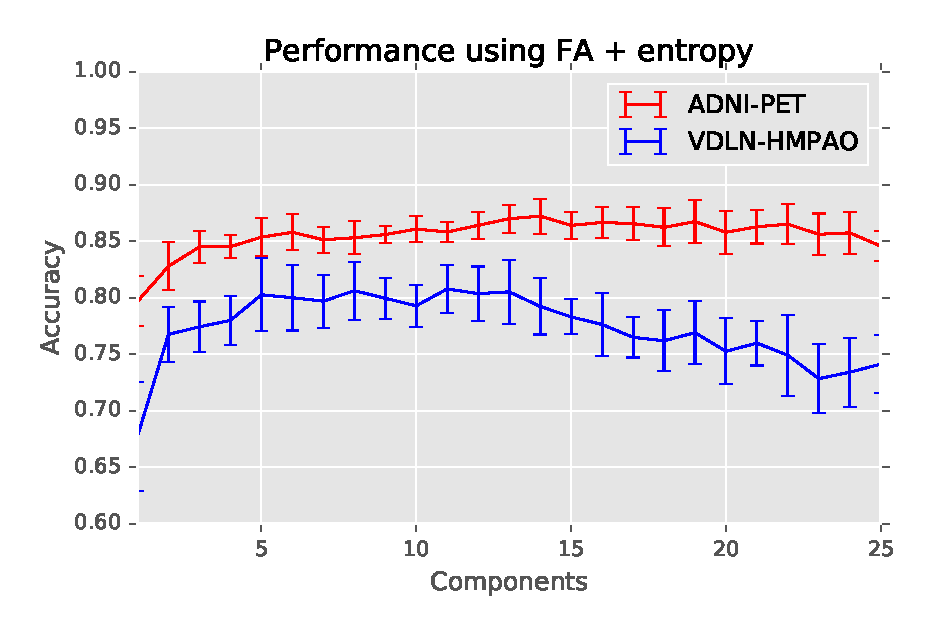
\includegraphics[width=0.49\linewidth]{Graphics/ch4/accuracyMeanSTD-FA_vsK_entropy_AD.eps}\label{fig:AD-AV-FA-ENTROPY-VSK}}
	
	\subfloat[]{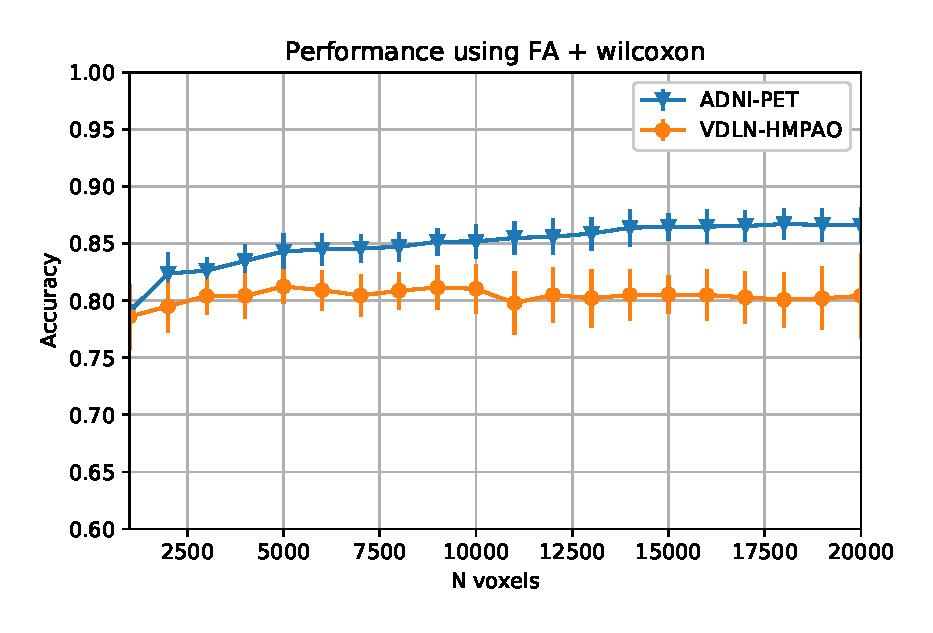
\includegraphics[width=0.49\linewidth]{Graphics/ch4/accuracyMeanSTD-FA_vsN_wilcoxon_AD.eps}\label{fig:AD-AV-FA-WILCOXON-VSN}}
	\subfloat[]{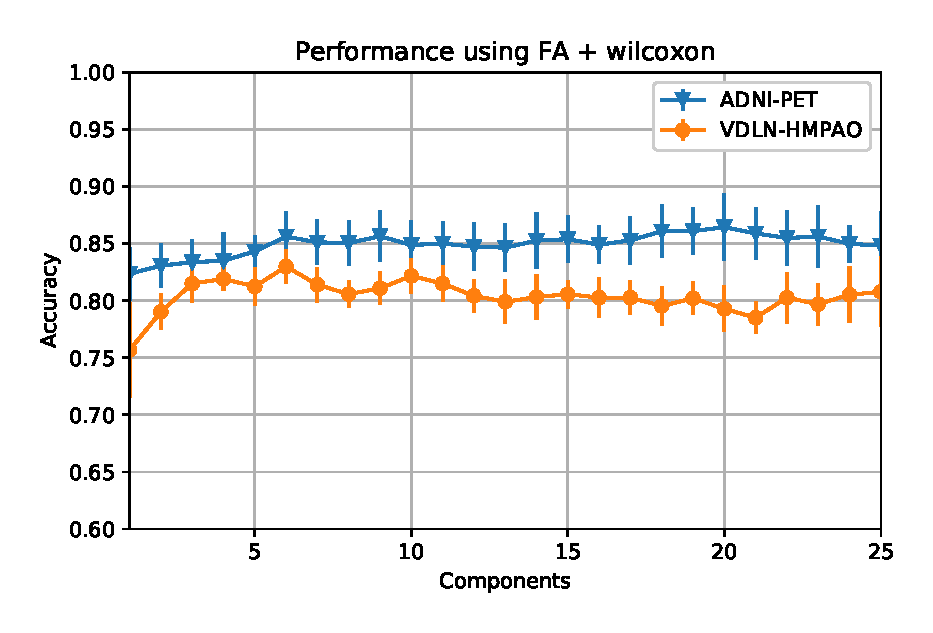
\includegraphics[width=0.49\linewidth]{Graphics/ch4/accuracyMeanSTD-FA_vsK_wilcoxon_AD.eps}\label{fig:AD-AV-FA-WILCOXON-VSK}}
	
	\caption{Average performance and standard deviation of the proposed system using the two \ac{AD} datasets, \ac{FA} and the three feature selection criteria: $t$-test (\protect\subref{fig:AD-AV-FA-TTEST-VSN} and \protect\subref{fig:AD-AV-FA-TTEST-VSK}), relative entropy (\protect\subref{fig:PKS-AV-FA-ENTROPY-VSN} and \protect\subref{fig:AD-AV-FA-ENTROPY-VSK}) and wilcoxon (\protect\subref{fig:AD-AV-FA-WILCOXON-VSN} and \protect\subref{fig:AD-AV-FA-WILCOXON-VSK}). } 
	\label{fig:accuracyMeanFA-AD}
\end{figure}

We can observe that the results are always better when using the ADNI-PET dataset than with the VDLN-HMPAO, and this is especially notorious when using the relative entropy selection criterion. The performance tends to slightly increase with the number of voxels selected, but it is not the case with the number of components. By looking at figures \ref{fig:AD-AV-FA-TTEST-VSK}, \ref{fig:AD-AV-FA-ENTROPY-VSK} and \ref{fig:AD-AV-FA-WILCOXON-VSK}, it seems that a relatively small number of components (approximately 6) is enough to obtain good performance, and afterwards, the performance holds or even decreases. 

\subsubsection{Independent Component Analysis}
In this section, we compute the results of applying \ac{ICA} to the ADNI-PET and VDLN-HMPAO datasets. Figure~\ref{fig:accuracyMeanICA-AD} depicts the average accuracy over the number of voxels or the number of components respectively for the different selection criteria. 

\begin{figure}
	\centering
	\subfloat[]{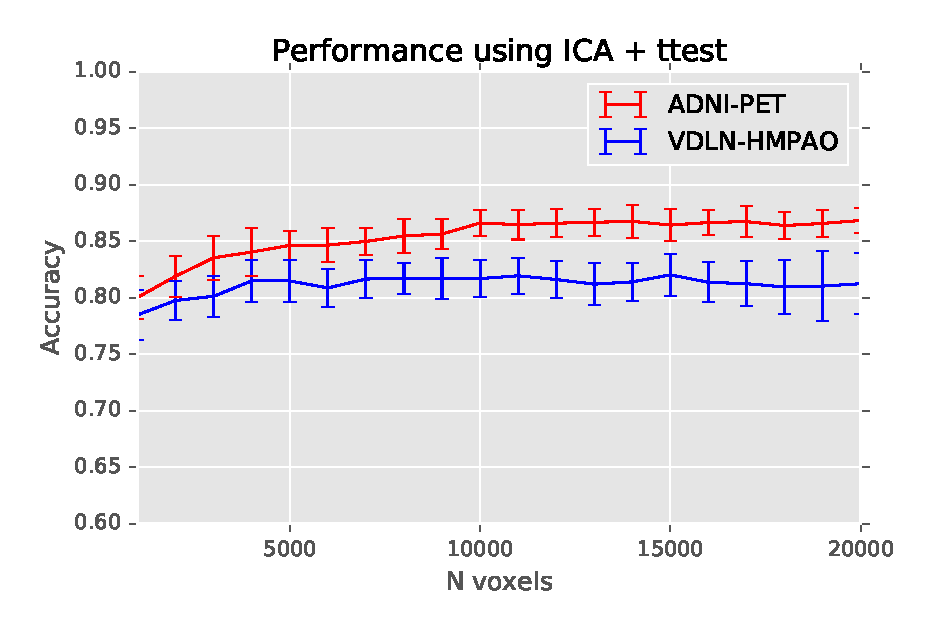
\includegraphics[width=0.49\linewidth]{Graphics/ch4/accuracyMeanSTD-ICA_vsN_ttest_AD.eps}\label{fig:AD-AV-ICA-TTEST-VSN}}
	\subfloat[]{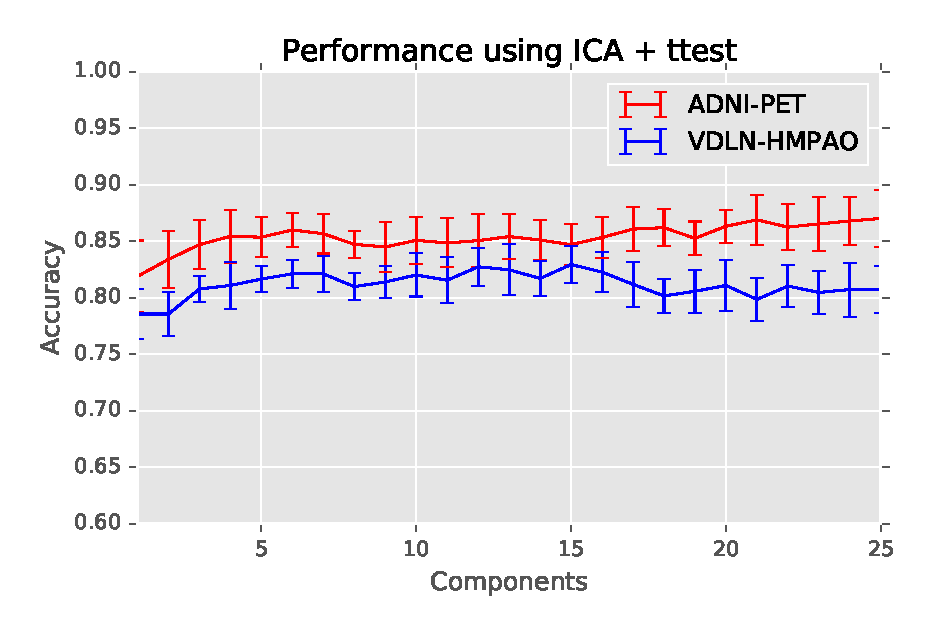
\includegraphics[width=0.49\linewidth]{Graphics/ch4/accuracyMeanSTD-ICA_vsK_ttest_AD.eps}\label{fig:AD-AV-ICA-TTEST-VSK}}
	
	\subfloat[]{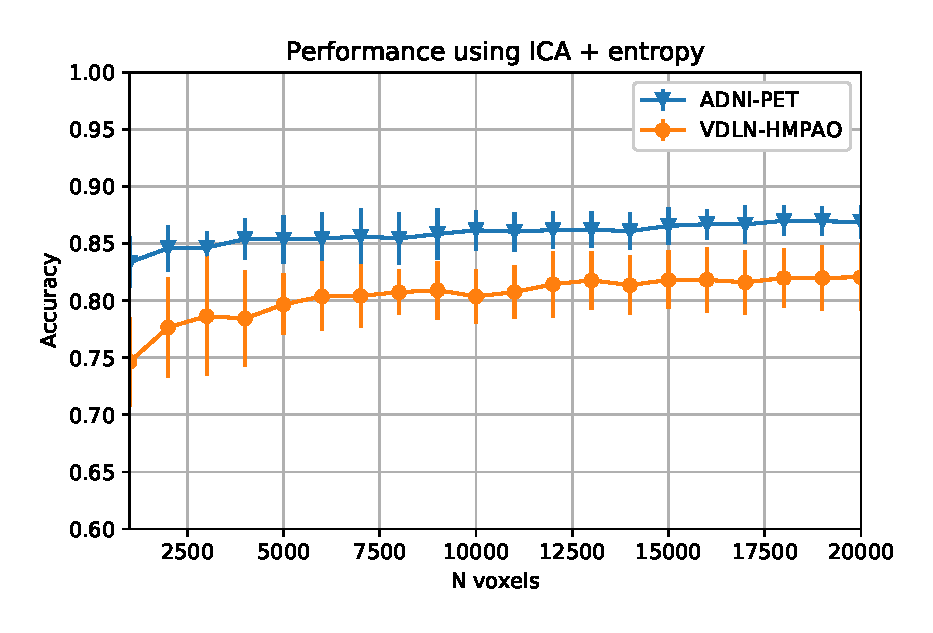
\includegraphics[width=0.49\linewidth]{Graphics/ch4/accuracyMeanSTD-ICA_vsN_entropy_AD.eps}\label{fig:AD-AV-ICA-ENTROPY-VSN}}
	\subfloat[]{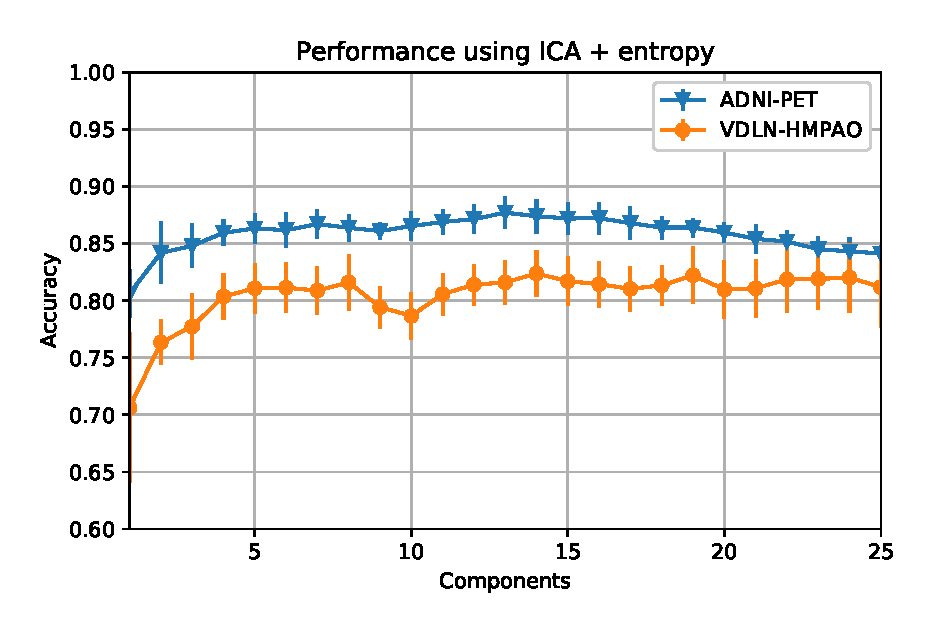
\includegraphics[width=0.49\linewidth]{Graphics/ch4/accuracyMeanSTD-ICA_vsK_entropy_AD.eps}\label{fig:AD-AV-ICA-ENTROPY-VSK}}
	
	\subfloat[]{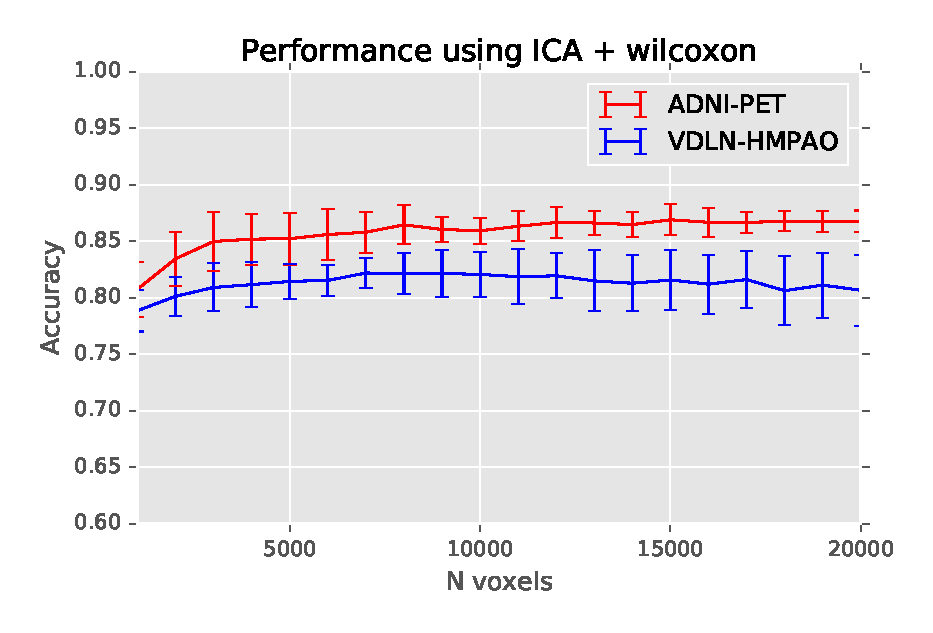
\includegraphics[width=0.49\linewidth]{Graphics/ch4/accuracyMeanSTD-ICA_vsN_wilcoxon_AD.eps}\label{fig:AD-AV-ICA-WILCOXON-VSN}}
	\subfloat[]{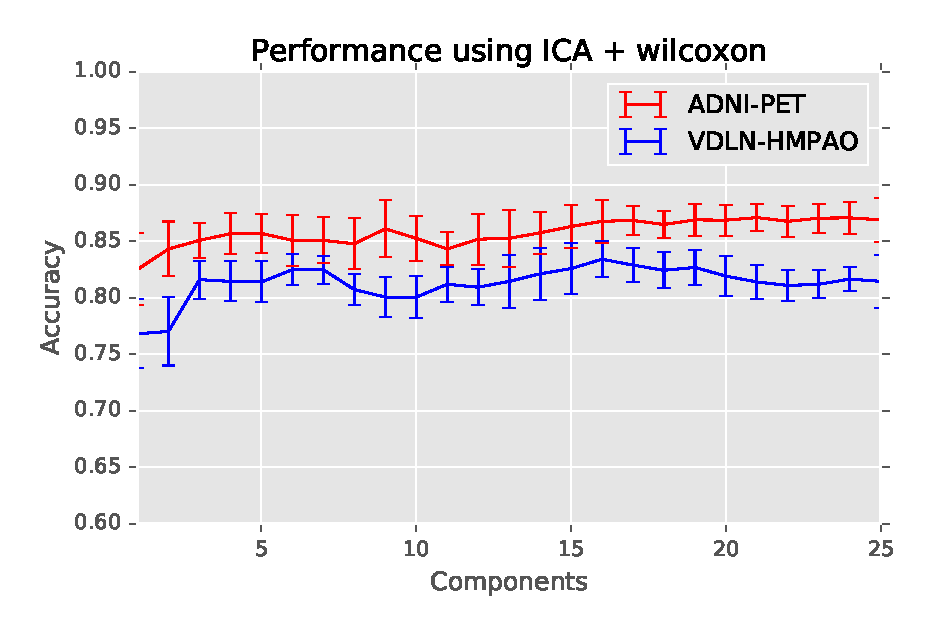
\includegraphics[width=0.49\linewidth]{Graphics/ch4/accuracyMeanSTD-ICA_vsK_wilcoxon_AD.eps}\label{fig:AD-AV-ICA-WILCOXON-VSK}}
	
	\caption{Average performance and standard deviation of the proposed system using the three \ac{AD} datasets, \ac{ICA} and the three feature selection criteria: $t$-test (\protect\subref{fig:AD-AV-ICA-TTEST-VSN} and \protect\subref{fig:AD-AV-ICA-TTEST-VSK}), relative entropy (\protect\subref{fig:AD-AV-ICA-ENTROPY-VSN} and \protect\subref{fig:AD-AV-ICA-ENTROPY-VSK}) and wilcoxon (\protect\subref{fig:AD-AV-ICA-WILCOXON-VSN} and \protect\subref{fig:AD-AV-ICA-WILCOXON-VSK}). } 
	\label{fig:accuracyMeanICA-AD}
\end{figure}

The case is similar to the one presented in Section~\ref{sec:results_FA_AD}, where the performance slightly improves when increasing the number of selected voxels. The performance is again better when using the ADNI-PET dataset than with the VDLN-HMPAO, although the behaviour is similar. 

The results change when varying the number of components. In this case, although good performance is obtained within the first 5 components in most cases, the performance does not decrease with a higher number, and sometimes increases (for example, in the case of \ac{ICA} and the $t$-test or the wilcoxon selection criteria). 

\subsubsection{At the Operation Point}
Now we focus on non-averaged values, the values for which our system is optimal: the operation point. 

\begin{figure}
	\centering
	\subfloat[]{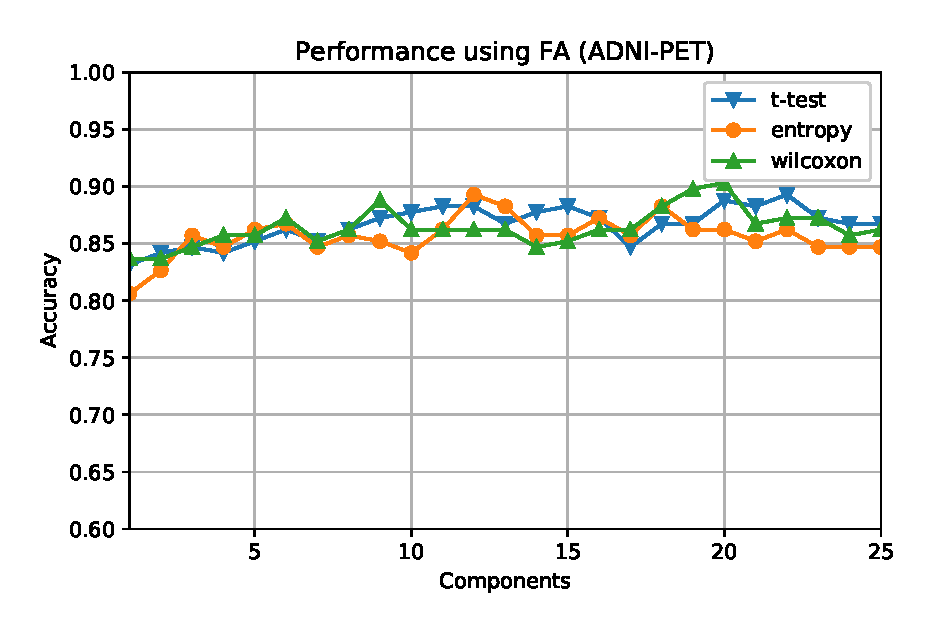
\includegraphics[width=0.49\linewidth]{Graphics/ch4/accuracyOP-FA_vsN_comparison_ADNI-PET.eps}\label{fig:ADNI-PET-FA-OP}}
	\subfloat[]{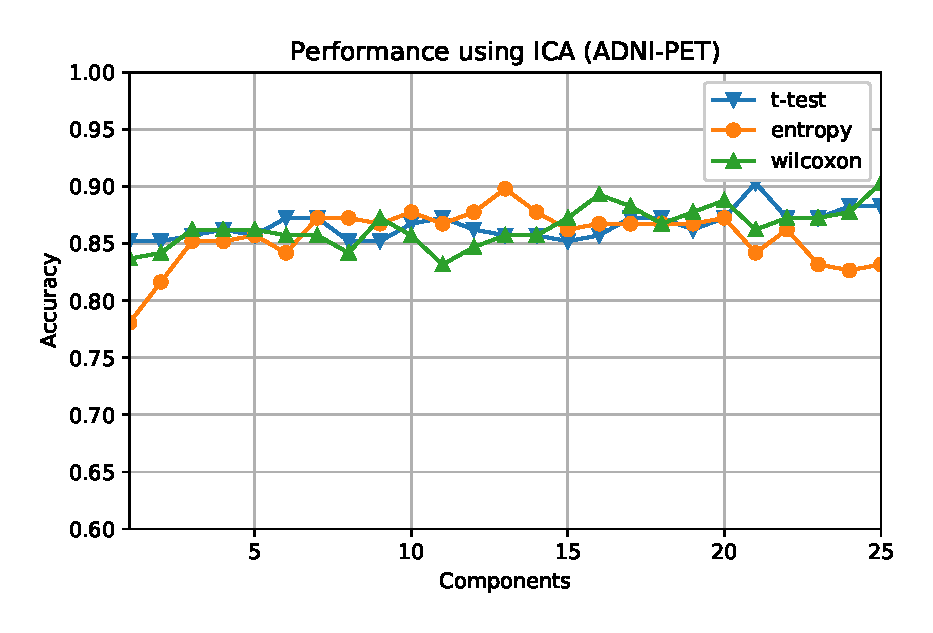
\includegraphics[width=0.49\linewidth]{Graphics/ch4/accuracyOP-ICA_vsN_comparison_ADNI-PET.eps}\label{fig:ADNI-PET-ICA-OP}}
	
	\subfloat[]{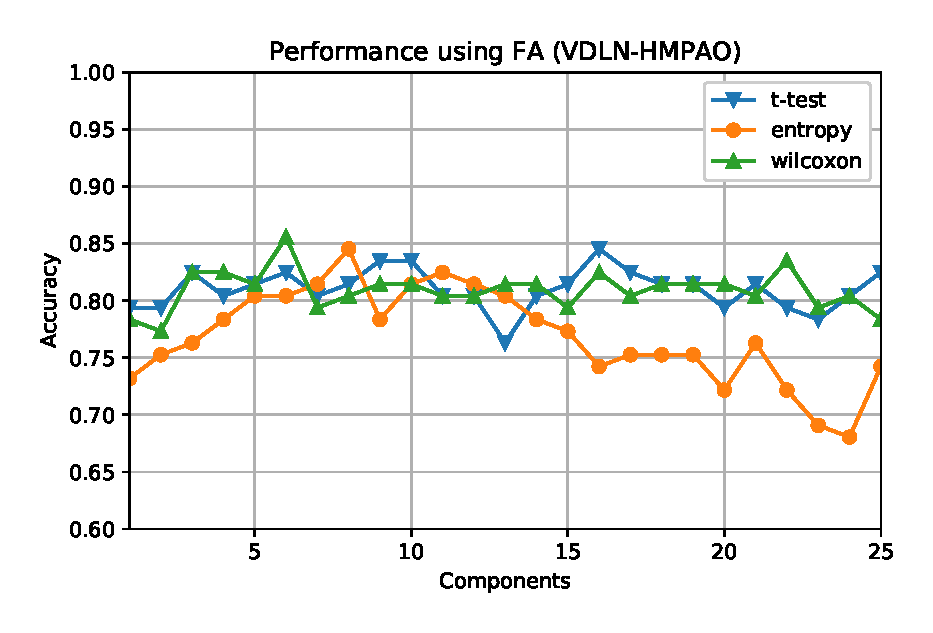
\includegraphics[width=0.49\linewidth]{Graphics/ch4/accuracyOP-FA_vsN_comparison_VDLN-HMPAO.eps}\label{fig:VDLN-HMPAO-FA-OP}}
	\subfloat[]{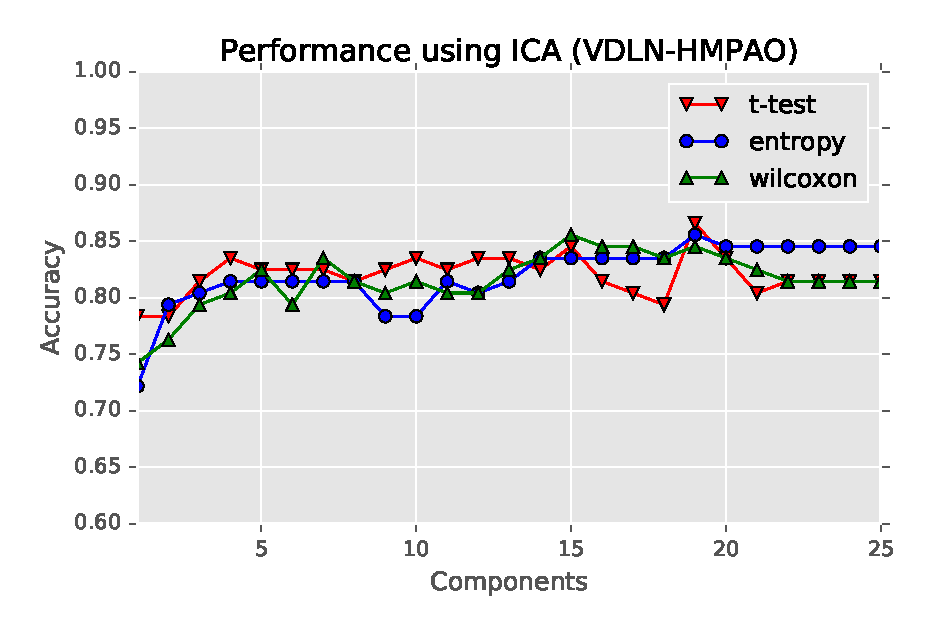
\includegraphics[width=0.49\linewidth]{Graphics/ch4/accuracyOP-ICA_vsN_comparison_VDLN-HMPAO.eps}\label{fig:VDLN-HMPAO-ICA-OP}}
	
	\caption{Performance of the proposed system using the two \ac{AD} datasets: ADNI-PET and VDLN-HMPAO at the operation point, and how they vary over the number of components used in the decomposition. } 
	\label{fig:accuracyOP-AD}
\end{figure}


\begin{table}
	\myfloatalign
	\begin{tabularx}{\linewidth}{Xllccc}
		\tableheadline{DB} & \tableheadline{Dec.} & \tableheadline{Criterion} & \tableheadline{Accuracy} & \tableheadline{Sensitivity} & \tableheadline{Specificity}\\
		\toprule
		\multirow{6}{1.7cm}{ADNI- PET} & \multirow{3}{*}{\ac{FA}} & t-test & $ 0.893 \pm 0.074 $ & $ 0.886 \pm 0.119 $ & $ 0.901 \pm 0.101 $ \\
		&  & entropy & $ 0.893 \pm 0.074 $ & $ 0.894 \pm 0.092 $ & $ 0.891 \pm 0.088 $ \\
		&  & wilcoxon & $ 0.903 \pm 0.066 $ & $ 0.917 \pm 0.079 $ & $ 0.891 \pm 0.082 $ \\
		\cline{2-6}
		& \multirow{3}{*}{\ac{ICA}} & t-test & $ 0.903 \pm 0.071 $ & $ 0.893 \pm 0.100 $ & $ 0.910 \pm 0.107 $ \\
		&  & entropy & $ 0.898 \pm 0.059 $ & $ 0.917 \pm 0.088 $ & $ 0.881 \pm 0.084 $ \\
		&  & wilcoxon & $ 0.903 \pm 0.066 $ & $ 0.906 \pm 0.097 $ & $ 0.901 \pm 0.094 $ \\ \midrule
		\multirow{6}{1.7cm}{VDLN- HMPAO} & \multirow{3}{*}{\ac{FA}} & t-test & $ 0.845 \pm 0.102 $ & $ 0.843 \pm 0.158 $ & $ 0.855 \pm 0.140 $ \\
		&  & entropy & $ 0.845 \pm 0.052 $ & $ 0.893 \pm 0.146 $ & $ 0.785 \pm 0.163 $ \\
		&  & wilcoxon & $ 0.856 \pm 0.084 $ & $ 0.857 \pm 0.137 $ & $ 0.855 \pm 0.151 $ \\
		\cline{2-6}
		& \multirow{3}{*}{\ac{ICA}} & t-test & $ 0.866 \pm 0.085 $ & $ 0.873 \pm 0.144 $ & $ 0.855 \pm 0.154 $ \\
		&  & entropy & $ 0.856 \pm 0.101 $ & $ 0.853 \pm 0.138 $ & $ 0.855 \pm 0.151 $ \\
		&  & wilcoxon & $ 0.856 \pm 0.086 $ & $ 0.857 \pm 0.156 $ & $ 0.855 \pm 0.160 $ \\
		\bottomrule
	\end{tabularx}
	\caption{Accuracy, sensitivity, specificity, and their standard deviation at the operation point for each method and its corresponding feature selection criterion, using two \protect\ac{AD} datasets. }
	\label{tab:featureAD}
\end{table}
\FloatBarrier
\subsection{Parkinson's Disease}


\subsubsection{Factor Analysis}
\begin{figure}
	\centering
	\subfloat[]{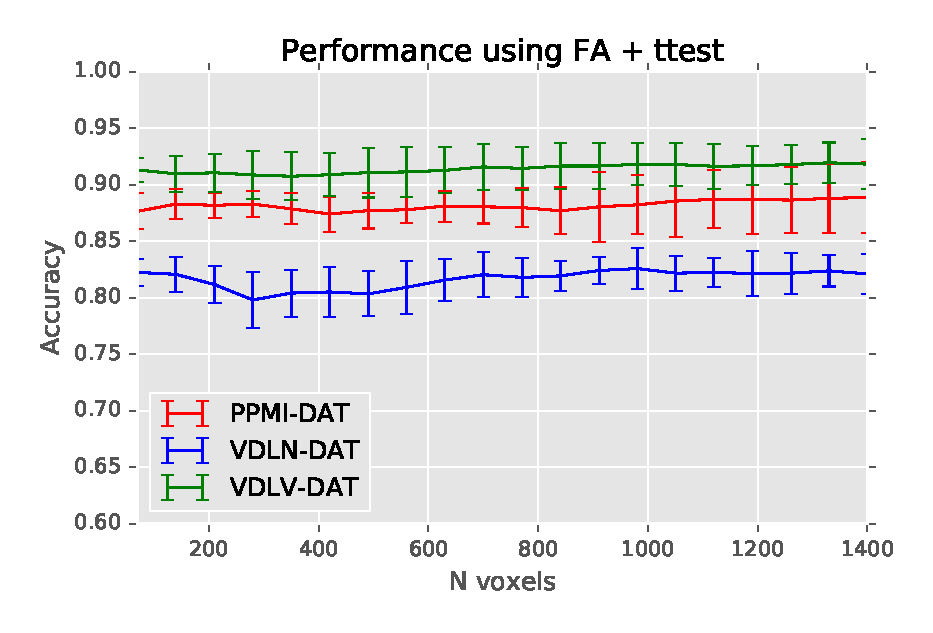
\includegraphics[width=0.49\linewidth]{Graphics/ch4/accuracyMeanSTD-FA_vsN_ttest_PKS.eps}\label{fig:PKS-AV-FA-TTEST-VSN}}
	\subfloat[]{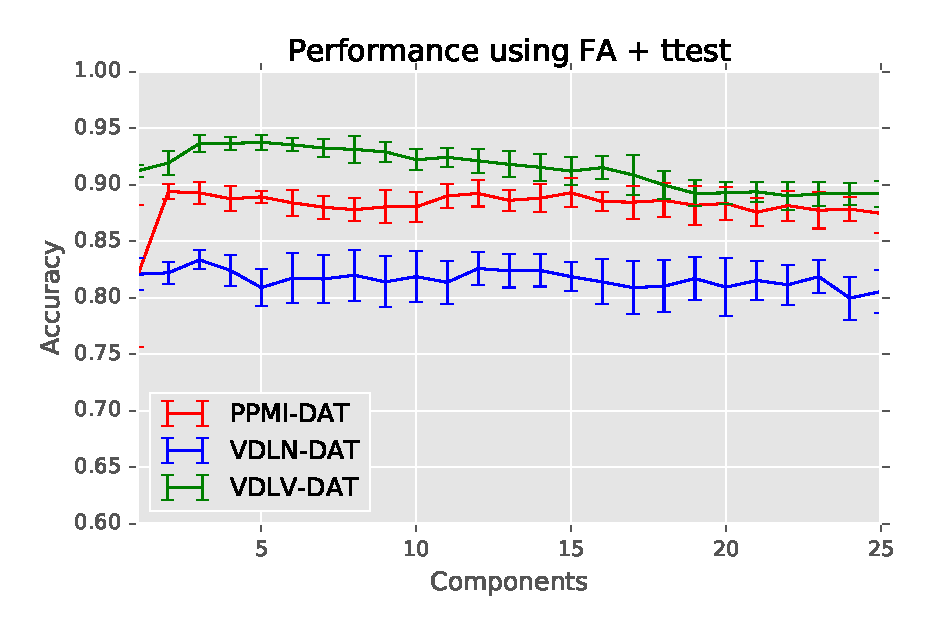
\includegraphics[width=0.49\linewidth]{Graphics/ch4/accuracyMeanSTD-FA_vsK_ttest_PKS.eps}\label{fig:PKS-AV-FA-TTEST-VSK}}
	
	\subfloat[]{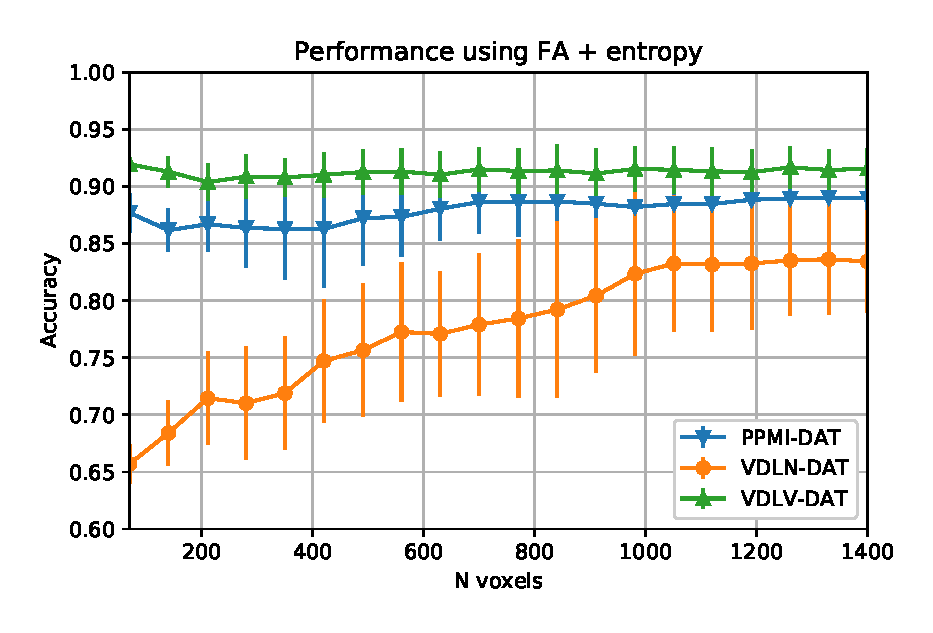
\includegraphics[width=0.49\linewidth]{Graphics/ch4/accuracyMeanSTD-FA_vsN_entropy_PKS.eps}\label{fig:PKS-AV-FA-ENTROPY-VSN}}
	\subfloat[]{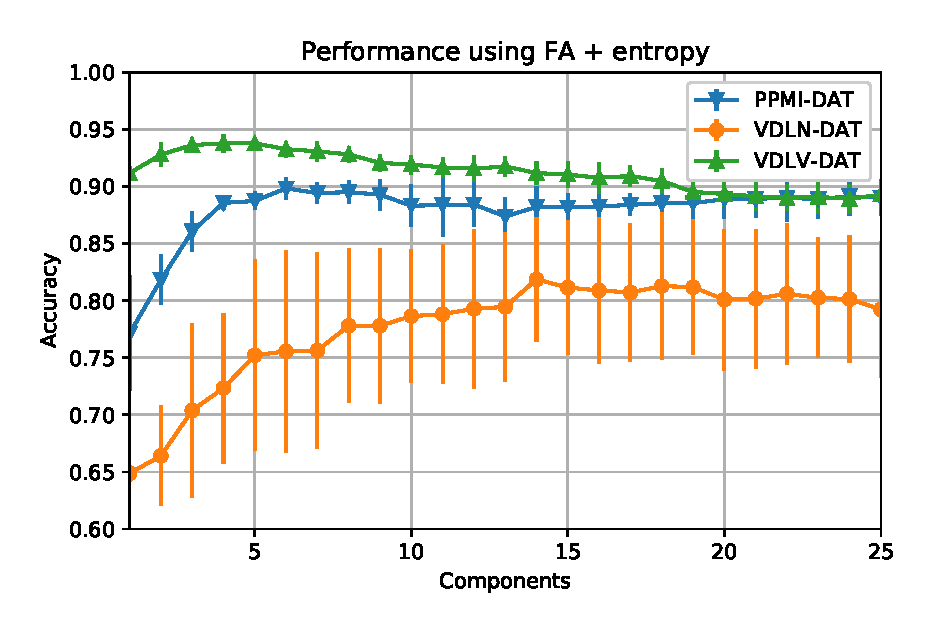
\includegraphics[width=0.49\linewidth]{Graphics/ch4/accuracyMeanSTD-FA_vsK_entropy_PKS.eps}\label{fig:PKS-AV-FA-ENTROPY-VSK}}
	
	\subfloat[]{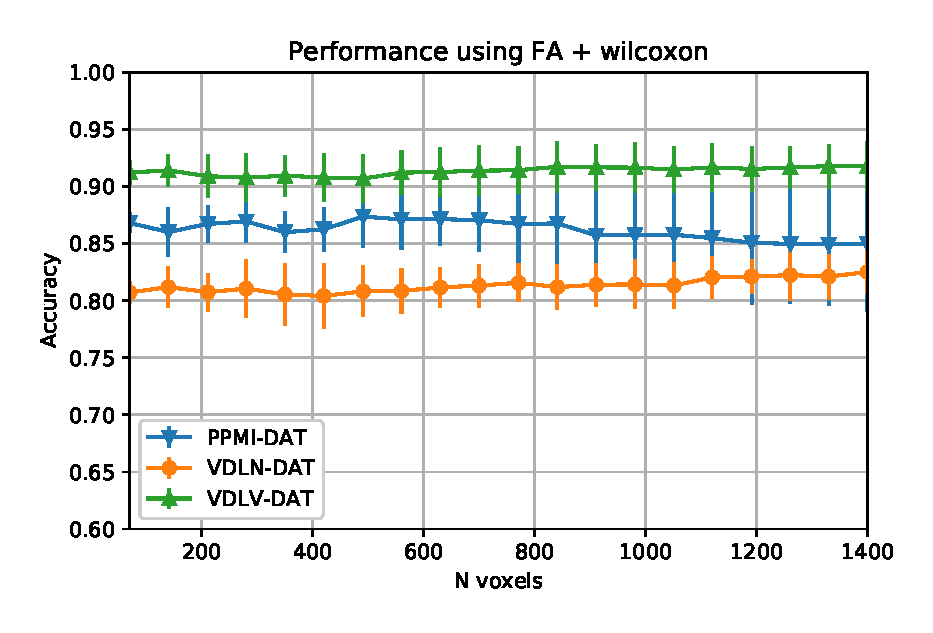
\includegraphics[width=0.49\linewidth]{Graphics/ch4/accuracyMeanSTD-FA_vsN_wilcoxon_PKS.eps}\label{fig:PKS-AV-FA-WILCOXON-VSN}}
	\subfloat[]{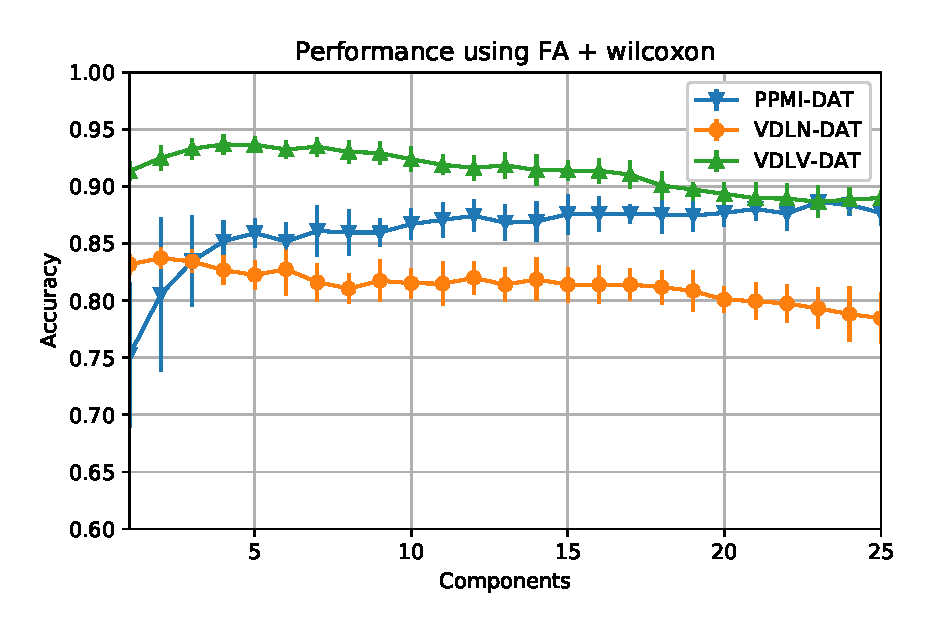
\includegraphics[width=0.49\linewidth]{Graphics/ch4/accuracyMeanSTD-FA_vsK_wilcoxon_PKS.eps}\label{fig:PKS-AV-FA-WILCOXON-VSK}}
	
	\caption{Average performance and standard deviation of the proposed system using the three \ac{PKS} datasets, \ac{FA} and the three feature selection criteria: $t$-test (\protect\subref{fig:PKS-AV-FA-TTEST-VSN} and \protect\subref{fig:PKS-AV-FA-TTEST-VSK}), relative entropy (\protect\subref{fig:PKS-AV-FA-ENTROPY-VSN} and \protect\subref{fig:PKS-AV-FA-ENTROPY-VSK}) and wilcoxon (\protect\subref{fig:PKS-AV-FA-WILCOXON-VSN} and \protect\subref{fig:PKS-AV-FA-WILCOXON-VSK}). } 
	\label{fig:accuracyMeanFA-PKS}
\end{figure}

\subsubsection{Independent Component Analysis}
\begin{figure}
	\subfloat[]{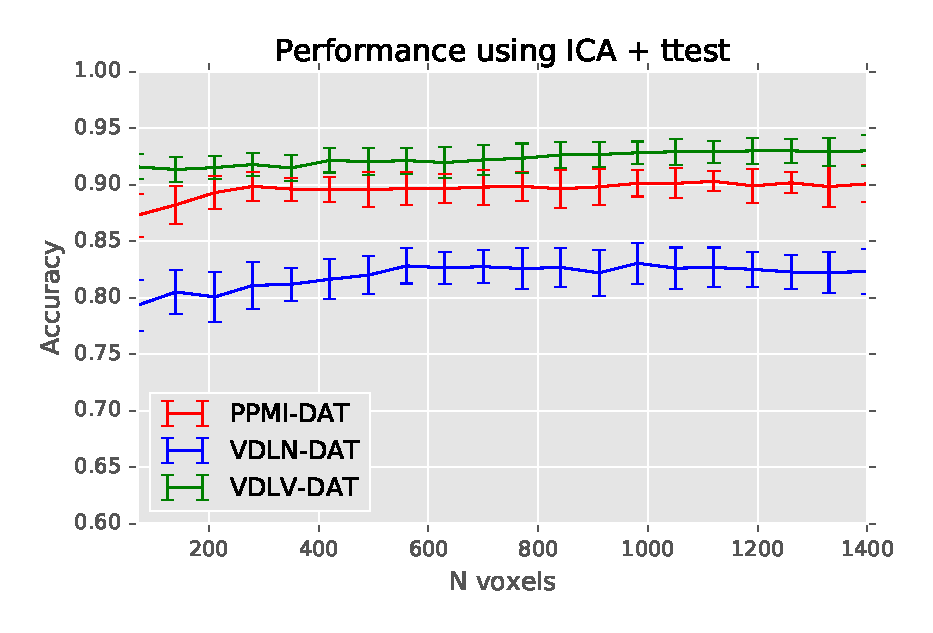
\includegraphics[width=0.49\linewidth]{Graphics/ch4/accuracyMeanSTD-ICA_vsN_ttest_PKS.eps}\label{fig:PKS-AV-ICA-TTEST-VSN}}
	\subfloat[]{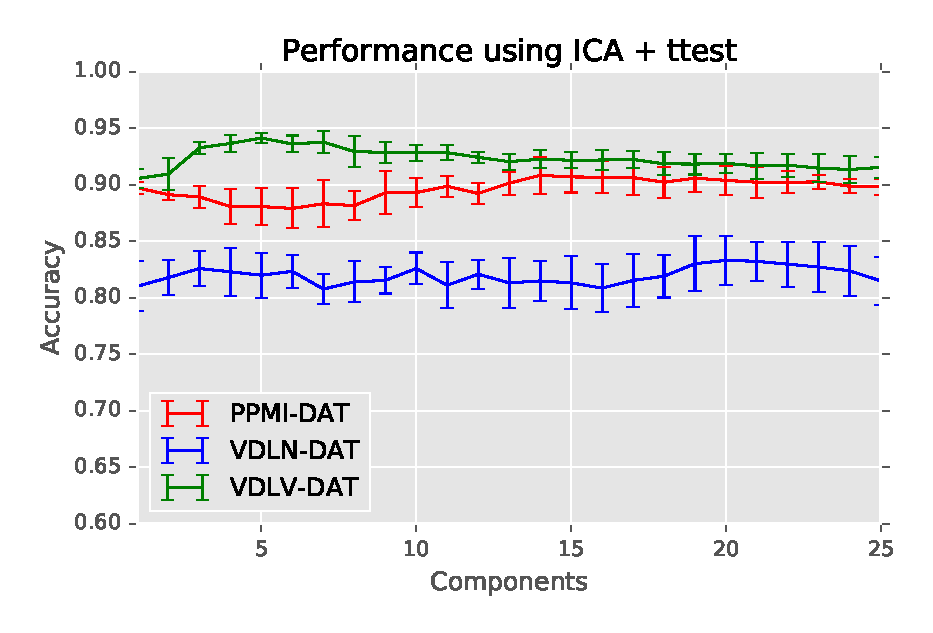
\includegraphics[width=0.49\linewidth]{Graphics/ch4/accuracyMeanSTD-ICA_vsK_ttest_PKS.eps}\label{fig:PKS-AV-ICA-TTEST-VSK}}
	
	\subfloat[]{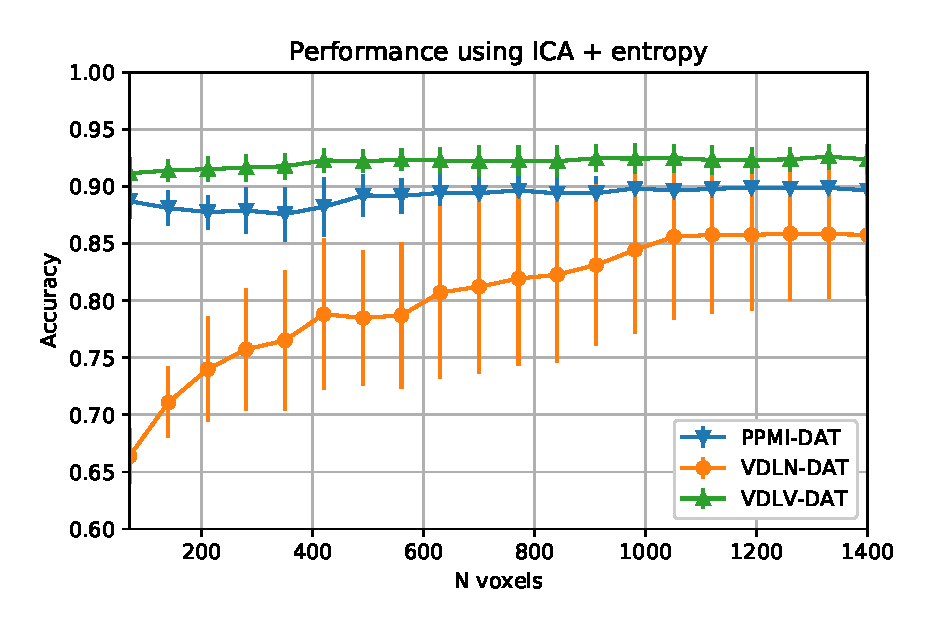
\includegraphics[width=0.49\linewidth]{Graphics/ch4/accuracyMeanSTD-ICA_vsN_entropy_PKS.eps}\label{fig:PKS-AV-ICA-ENTROPY-VSN}}
	\subfloat[]{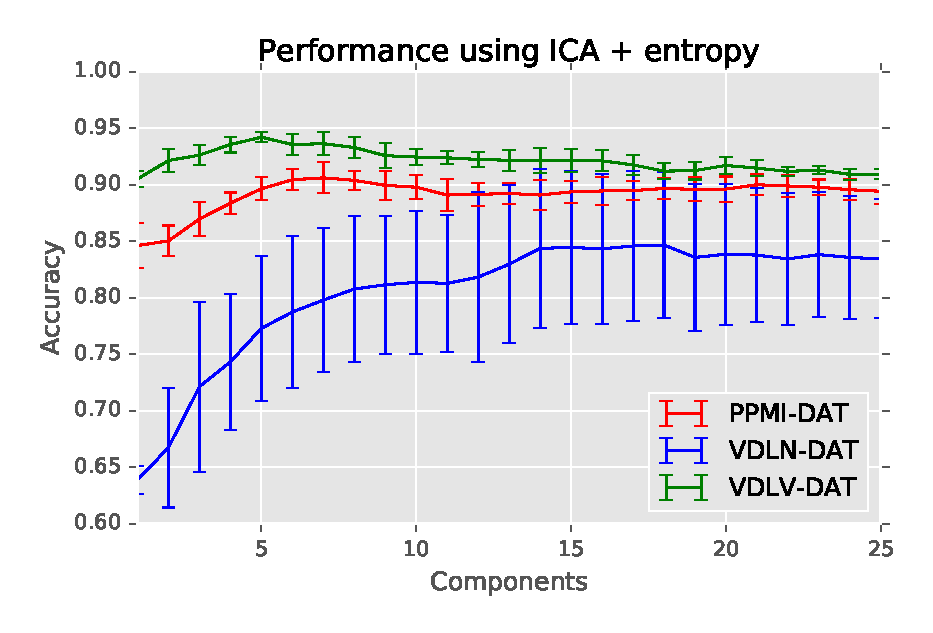
\includegraphics[width=0.49\linewidth]{Graphics/ch4/accuracyMeanSTD-ICA_vsK_entropy_PKS.eps}\label{fig:PKS-AV-ICA-ENTROPY-VSK}}
	
	\subfloat[]{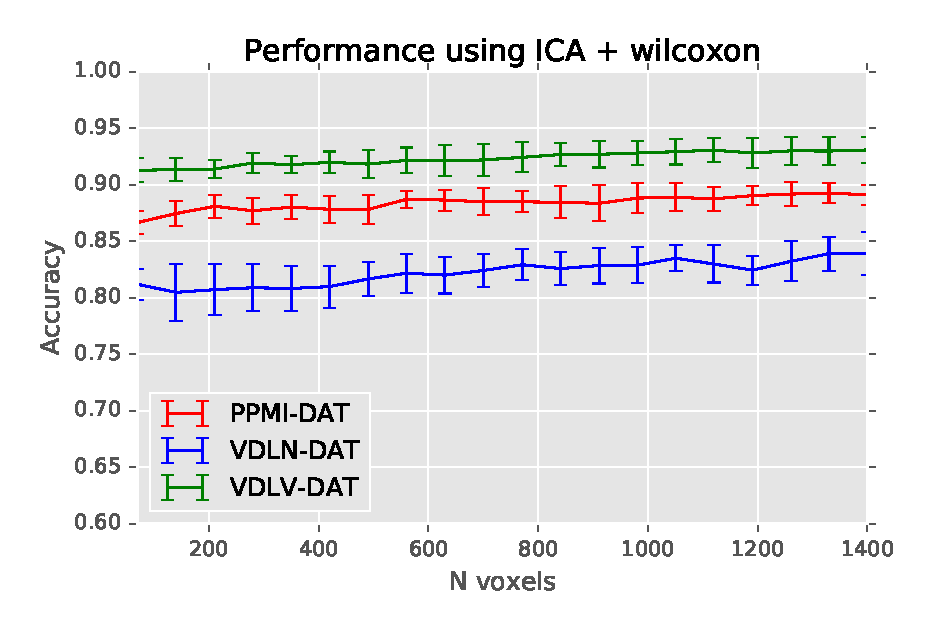
\includegraphics[width=0.49\linewidth]{Graphics/ch4/accuracyMeanSTD-ICA_vsN_wilcoxon_PKS.eps}\label{fig:PKS-AV-ICA-WILCOXON-VSN}}
	\subfloat[]{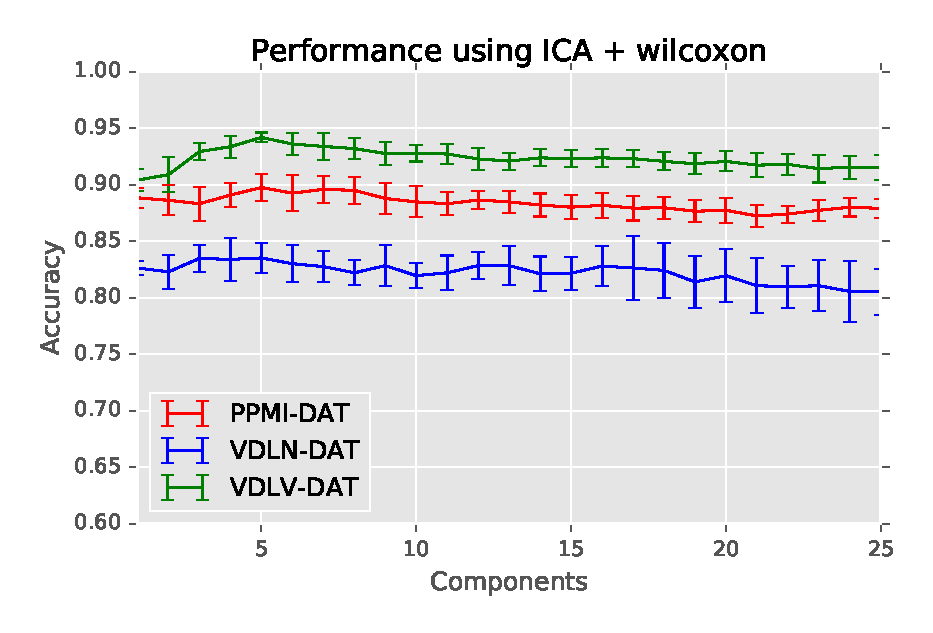
\includegraphics[width=0.49\linewidth]{Graphics/ch4/accuracyMeanSTD-ICA_vsK_wilcoxon_PKS.eps}\label{fig:PKS-AV-ICA-WILCOXON-VSK}}
	
	\caption{Average performance and standard deviation of the proposed system using the three \ac{PKS} datasets, \ac{ICA} and the three feature selection criteria: $t$-test (\protect\subref{fig:PKS-AV-ICA-TTEST-VSN} and \protect\subref{fig:PKS-AV-ICA-TTEST-VSK}), relative entropy (\protect\subref{fig:PKS-AV-ICA-ENTROPY-VSN} and \protect\subref{fig:PKS-AV-ICA-ENTROPY-VSK}) and wilcoxon (\protect\subref{fig:PKS-AV-ICA-WILCOXON-VSN} and \protect\subref{fig:PKS-AV-ICA-WILCOXON-VSK}). } 
	\label{fig:accuracyMeanICA-PKS}
\end{figure}


\subsubsection{At the Operation Point}

\begin{figure}
	\subfloat[]{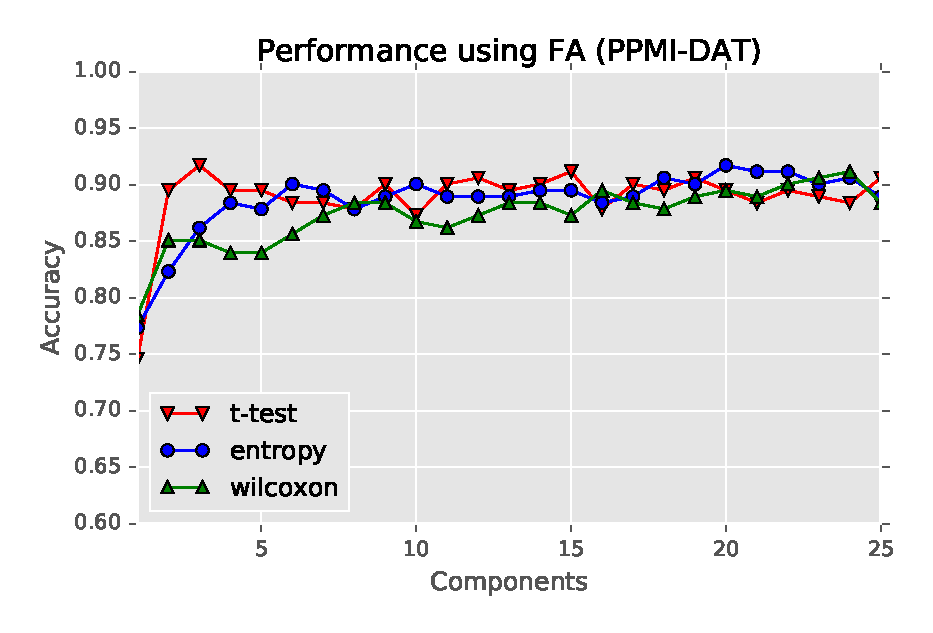
\includegraphics[width=0.49\linewidth]{Graphics/ch4/accuracyOP-FA_vsN_comparison_PPMI-DAT.eps}\label{fig:PPMI-DAT-FA-OP}}
	\subfloat[]{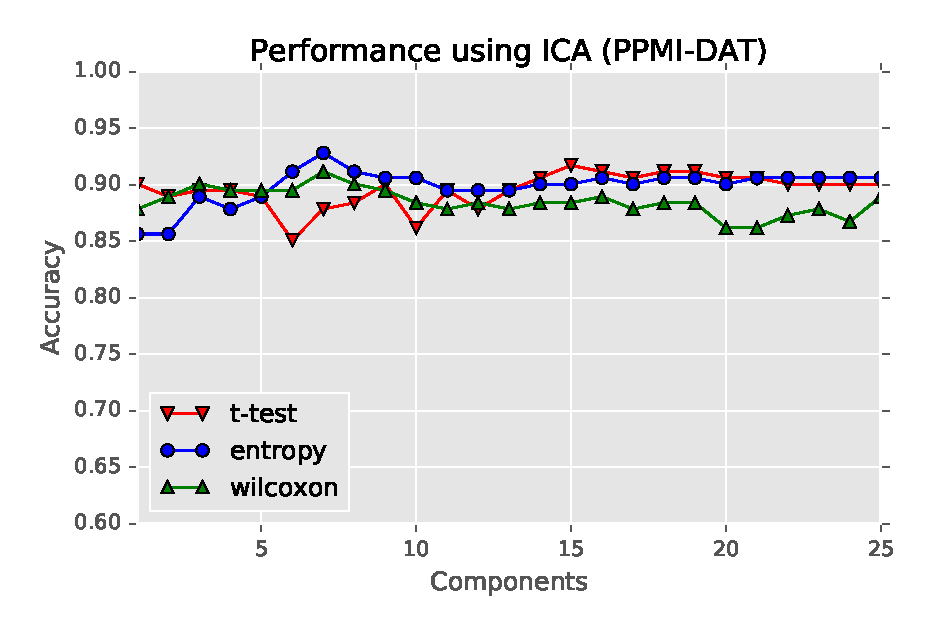
\includegraphics[width=0.49\linewidth]{Graphics/ch4/accuracyOP-ICA_vsN_comparison_PPMI-DAT.eps}\label{fig:PPMI-DAT-ICA-OP}}
	
	\subfloat[]{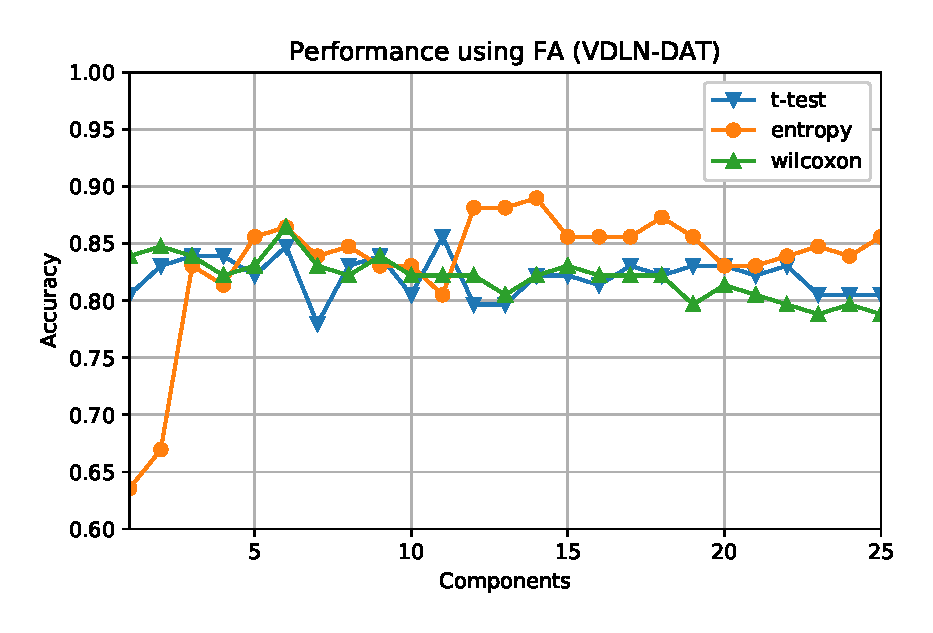
\includegraphics[width=0.49\linewidth]{Graphics/ch4/accuracyOP-FA_vsN_comparison_VDLN-DAT.eps}\label{fig:VDLN-DAT-FA-OP}}
	\subfloat[]{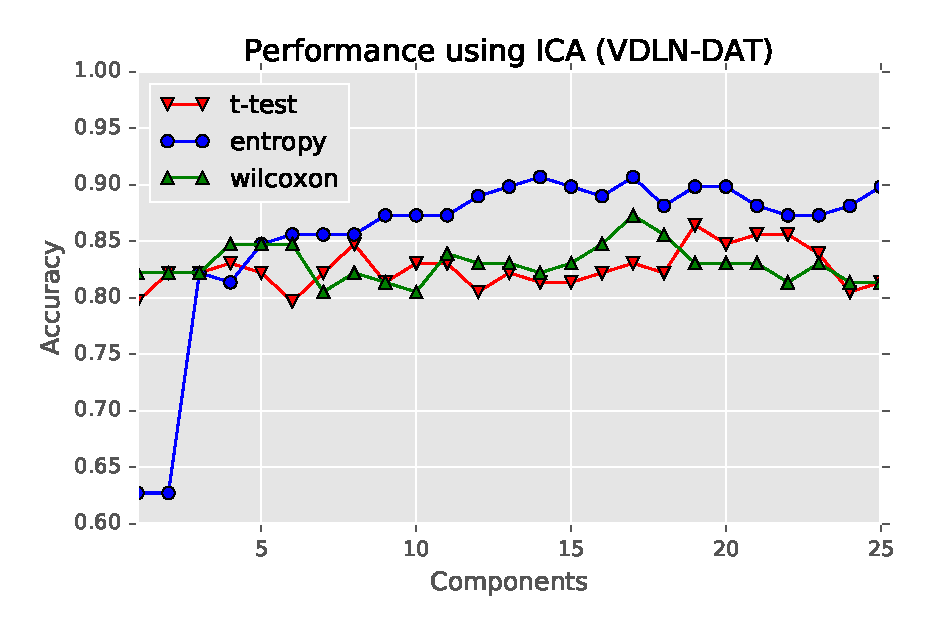
\includegraphics[width=0.49\linewidth]{Graphics/ch4/accuracyOP-ICA_vsN_comparison_VDLN-DAT.eps}\label{fig:VDLN-DAT-ICA-OP}}
	
	\subfloat[]{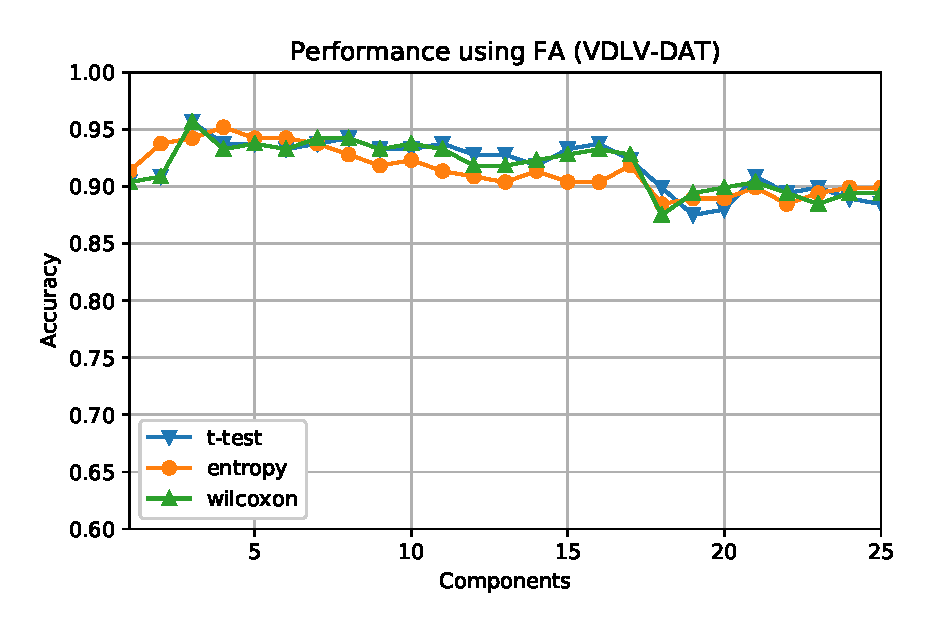
\includegraphics[width=0.49\linewidth]{Graphics/ch4/accuracyOP-FA_vsN_comparison_VDLV-DAT.eps}\label{fig:VDLV-DAT-FA-OP}}
	\subfloat[]{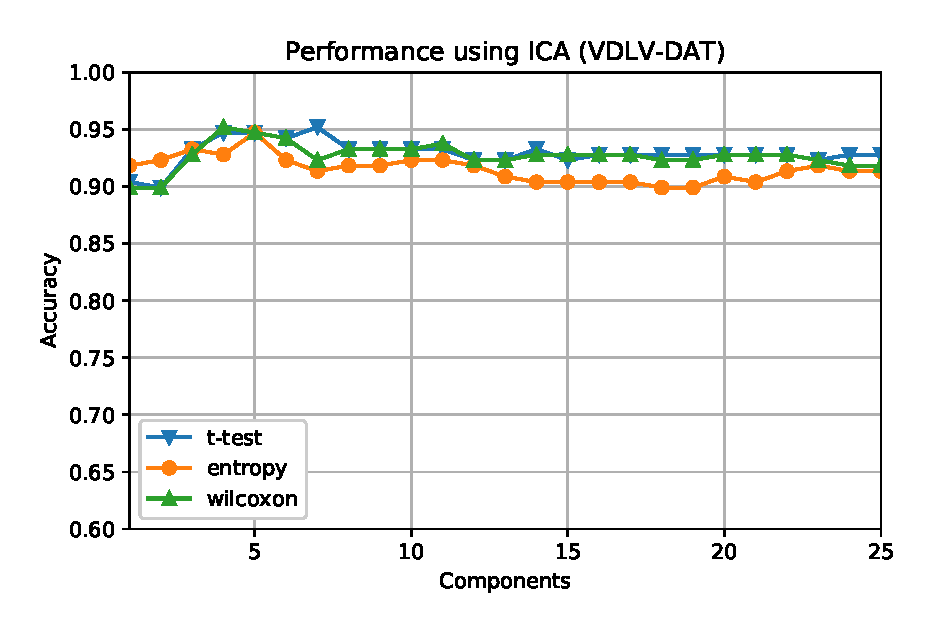
\includegraphics[width=0.49\linewidth]{Graphics/ch4/accuracyOP-ICA_vsN_comparison_VDLV-DAT.eps}\label{fig:VDLV-DAT-ICA-OP}}
	
	\caption{Performance of the proposed system using the two \ac{PKS} datasets: PPMI-DAT, VDLN-DAT and VDLV-DAT at the operation point, and how they vary over the number of components used in the decomposition. } 
	\label{fig:accuracyOP-PKS}
\end{figure}


\begin{table}
	\begin{tabularx}{\linewidth}{Xllccc}
		\tableheadline{DB} & \tableheadline{Dec.} & \tableheadline{Criterion} & \tableheadline{Accuracy} & \tableheadline{Sensitivity} & \tableheadline{Specificity}\\
		\toprule
		\multirow{6}{1.7cm}{VDLN-DAT} & \multirow{3}{*}{\ac{FA}} & t-test & $ 0.856 \pm 0.111 $ & $ 0.887 \pm 0.178 $ & $ 0.795 \pm 0.164 $ \\
		&  & entropy & $ 0.890 \pm 0.098 $ & $ 0.875 \pm 0.118 $ & $ 0.910 \pm 0.116 $ \\
		&  & wilcoxon & $ 0.864 \pm 0.070 $ & $ 0.916 \pm 0.114 $ & $ 0.780 \pm 0.183 $ \\
		\cline{2-6}
		& \multirow{3}{*}{\ac{ICA}} & t-test & $ 0.864 \pm 0.101 $ & $ 0.873 \pm 0.174 $ & $ 0.840 \pm 0.166 $ \\
		&  & entropy & $ 0.907 \pm 0.075 $ & $ 0.889 \pm 0.124 $ & $ 0.935 \pm 0.131 $ \\
		&  & wilcoxon & $ 0.873 \pm 0.108 $ & $ 0.859 \pm 0.181 $ & $ 0.890 \pm 0.151 $ \\
		\midrule
		\multirow{6}{1.7cm}{VDLV-DAT} & \multirow{3}{*}{\ac{FA}} & t-test & $ 0.957 \pm 0.033 $ & $ 0.940 \pm 0.066 $ & $ 0.973 \pm 0.065 $ \\
		&  & entropy & $ 0.952 \pm 0.037 $ & $ 0.940 \pm 0.066 $ & $ 0.964 \pm 0.064 $ \\
		&  & wilcoxon & $ 0.957 \pm 0.033 $ & $ 0.940 \pm 0.066 $ & $ 0.973 \pm 0.065 $ \\
		\cline{2-6}
		& \multirow{3}{*}{\ac{ICA}} & t-test & $ 0.952 \pm 0.037 $ & $ 0.940 \pm 0.066 $ & $ 0.964 \pm 0.064 $ \\
		&  & entropy & $ 0.947 \pm 0.045 $ & $ 0.940 \pm 0.066 $ & $ 0.955 \pm 0.076 $ \\
		&  & wilcoxon & $ 0.952 \pm 0.037 $ & $ 0.940 \pm 0.066 $ & $ 0.964 \pm 0.064 $ \\
		\midrule
		\multirow{6}{1.7cm}{PPMI-DAT} & \multirow{3}{*}{\ac{FA}} & t-test & $ 0.917 \pm 0.037 $ & $ 0.918 \pm 0.095 $ & $ 0.918 \pm 0.091 $ \\
		&  & entropy & $ 0.917 \pm 0.060 $ & $ 0.918 \pm 0.076 $ & $ 0.921 \pm 0.120 $ \\
		&  & wilcoxon & $ 0.912 \pm 0.056 $ & $ 0.927 \pm 0.098 $ & $ 0.889 \pm 0.102 $ \\
		\cline{2-6}
		& \multirow{3}{*}{\ac{ICA}} & t-test & $ 0.917 \pm 0.056 $ & $ 0.900 \pm 0.095 $ & $ 0.948 \pm 0.109 $ \\
		&  & entropy & $ 0.928 \pm 0.055 $ & $ 0.909 \pm 0.091 $ & $ 0.961 \pm 0.090 $ \\
		&  & wilcoxon & $ 0.912 \pm 0.070 $ & $ 0.909 \pm 0.100 $ & $ 0.920 \pm 0.118 $ \\
		\bottomrule
		\end{tabularx}
		\caption{Accuracy, sensitivity, specificity, and their standard deviation at the operation point for each method and its corresponding feature selection criterion, using three \protect\ac{PKS} datasets }
		\label{tab:featurePKS}
\end{table}

\section{Discussion}